%% LyX 2.2.2 created this file.  For more info, see http://www.lyx.org/.
%% Do not edit unless you really know what you are doing.
\documentclass[oneside,english,brazil,11pt,a4paper,openright,titlepage]{book}
\setcounter{secnumdepth}{3}
\setcounter{tocdepth}{3}
\usepackage{array}
\usepackage{graphicx}
\usepackage[utf8]{inputenc}

\makeatletter

%%%%%%%%%%%%%%%%%%%%%%%%%%%%%% LyX specific LaTeX commands.
%% Because html converters don't know tabularnewline
\providecommand{\tabularnewline}{\\}

%%%%%%%%%%%%%%%%%%%%%%%%%%%%%% User specified LaTeX commands.
% Classe alternativa, apropriada para impressão frente-verso. Inclui páginas em branco
% de forma que capítulos sempre tenham início na página à direita:
% \documentclass[11pt,a4paper,openright,titlepage]{book}

\usepackage[T1]{fontenc}
\usepackage{ft4unb_MKT}
\usepackage[portuguese]{babel}
\@ifundefined{showcaptionsetup}{}{%
 \PassOptionsToPackage{caption=false}{subfig}}
\usepackage{subfig}
\makeatother

\usepackage{babel}

%%%%%%% My Includes %%%%%%%
\usepackage[hidelinks]{hyperref}
\usepackage{float}


\begin{document}
%CAPA
\grau{Engenheiro Mecatrônico}{Engenheiro} \tipodemonografia{Trabalho de Graduação}

% Título do trabalho (nao deletar linhas. Caso desejado, deixar em branco)
\titulolinhai{Implementação de Controle Fuzzy} 
\titulolinhaii{Em CLP Industrial} 
\titulolinhaiii{} 
\titulolinhaiv{}
\tituloingles{Fuzzy Control Implementation in Industrial CLP}

%Autores
\autori{Jhonantans Moraes Rocha} 
\autorii{} % deixar em branco se não houver segundo autor. 
\autoriii{} % deixar em branco se não houver terceiro autor. 

\capaprincipal

%CONTRA CAPA

%Membros da banca (até 5 membros) 
\membrodabancai{Prof. Eduardo Stockler Tognetti, ENE/UnB} \membrodabancaifuncao{Orientador} 
\membrodabancaii{Prof. Nome, Dept/Univ} \membrodabancaiifuncao{Co-Orientador}
\membrodabancaiii{Prof. Nome, Dept/Univ} \membrodabancaiiifuncao{Examinador Externo} 
\membrodabancaiv{Prof. Nome, Dept/Univ} \membrodabancaivfuncao{Examinador Interno} 
\membrodabancav{} \membrodabancavfuncao{}

%Data de defesa: dia, mês e ano. 
\dia{14} \mes{dezembro} \ano{2016}

\capaassinaturas

%FICHA CATALOGRAFICA

%Sobrenome, Nome Completo 
\autorcatalogo{Rocha, Jhonantans Moraes} 
%Sobrenome, Iniciais 
\autorabreviadocatalogo{Rocha, J.M.} 
%Número de páginas
\numeropaginascatalogo{60p.} 
\palavraschavecatalogoi{Fuzzy} 
\palavraschavecatalogoii{Controle} 
\palavraschavecatalogoiii{Quatro-Tanques} 
\palavraschavecatalogoiv{CLP} 
%Número da publicação (fornecido pelo departamento após a defesa) 
\publicacao{TG-002/2016}

\fichacatalografica

%DEDICATORIA
\frontmatter
% Texto primeiro autor 
\dedicatoriaautori{Dedicatória do autor 1}
% Texto segundo autor
\dedicatoriaautorii{Dedicatória do autor 2}
% Texto terceiro autor
\dedicatoriaautoriii{Dedicatória do autor 3}

\dedicatoria

%AGRADECIMENTOS
% Texto primeiro autor 
\agradecimentosautori{Primeira página de agradecimentos} 
% Conteudo da segunda pagina (caso agradecimentos sejam muito extensos)
\agradecimentosautorcont{}
% Texto segundo autor
\agradecimentosautorii{}
% Texto terceiro autor
\agradecimentosautoriii{}

\agradecimentos

\selectlanguage{english}%
%PORTUGUESE
\resumo{Resumo}{

Resumo em português.

}
%ENGLISH
\vspace*{2cm}
\resumo{Abstract}{

Abstract in english.

}\selectlanguage{brazil}%



\sumario

\listadefiguras

\listadetabelas

\selectlanguage{english}%

\chapter*{Lista de Símbolos}

\subsection*{Símbolos Latinos}

\begin{tabular}{>{\centering}p{0.1\textwidth}l}
$v_i$ & Tensão aplicada à Bomba $i$ \\ \tabularnewline
$k_i$ & Constante de Fluxo da Bomba $i$ \\ \tabularnewline
$g$ & Constante Aceleração da Gravidade \\ \tabularnewline
$H_i$ & Altura do Tanque $i$\\ \tabularnewline
$h_i$ & Altura do fluído do Tanque $i$\\ \tabularnewline
$A_i$ & Área da secção transversal do Tanque $i$\\ \tabularnewline
$a_i$ & Área do orifício de saída do Tanque $i$\\ \tabularnewline
\tabularnewline
\end{tabular}

\subsection*{Símbolos Gregos}

\begin{tabular}{>{\centering}p{0.1\textwidth}l}
$\gamma_i$ & Abertura da válvula $i$\\ \tabularnewline
\tabularnewline
\end{tabular}\selectlanguage{brazil}%



\selectlanguage{english}%

\chapter*{Notação}

Neste trabalho vetores são representados por letras minúsculas em
negrito. Matrizes são representadas por letras maiúsculas em negrito.
Já espaços e conjuntos em geral são representados por letras maiúsculas
caligráficas. \selectlanguage{brazil}%



%CORPO PRINCIPAL
\mainmatter 
\setcounter{page}{1} \pagestyle{plain} 

\selectlanguage{english}%

\chapter{Introdução} \label{capIntrod}
\epigraph{Não há assunto tão velho que não possa ser dito algo de novo sobre ele.}{Fiodor Dostoievski}

Desenvolver controladores para sistemas não-lineares é quase sempre uma tarefa dispendiosa e complexa. Para plantas multivariáveis não-lineares este desafio é ainda maior. É por este motivo que é prática comum recorrer-se à linearização das equações que as descrevem, obtendo uma aproximação do sistema inicial num formato que se encaixa às teorias de controle convencionais para sistemas lineares.

Esta linearização simples, realizada por meio da série de Taylor, resulta numa aproximação local do sistema não-linear. No entanto, à medida que as variáveis controladas e manipuladas se afastam deste ponto de operação, condição na qual foi realizada a linearização, o modelo passa a se afastar da planta real.

Neste cenário, a abordagem fuzzy figura como excelente ferramenta para solução destes desvios. Aparecendo pela primeira vez nos trabalhos de Zadeh \cite{zadeh}, foi desenvolvida para aplicações em modelagem de sistemas nos trabalhos de Takagi e Sugeno \cite{takagiSugeno}. Seus métodos consistem na linearização convencional do sistema em múltiplos pontos escolhidos criteriosamente, baseados em um conjunto de métricas relevantes para o problema em questão. A partir daí desenvolve-se um conjunto de regras para determinar o grau de conformidade de cada estado do sistema à cada um dos pontos pré-modelados. Utiliza-se então como modelo a soma (uma interpolação) dos múltiplos modelos iniciais ponderada por estes coeficiente de pertinência. 

O objeto de estudo deste trabalho é o sistema de quatro tanques, desenvolvido por Karl Johansson \cite{johansson2} com o objetivo didático de demonstrar de forma ilustrativa conceitos e propriedades de sistemas com múltiplas entradas e saídas (MIMO, do inglês \textit{Multiple Input, Multiple Output}). Ele consiste em quatro tanques interconectados, um reservatório inferior, duas válvulas esferas e duas bombas de corrente contínua que bombeiam o fluido do reservatório inferior para os tanques de forma cruzada, de acordo com a razão entre os fluxos definida pela posição das válvulas. O sistema de quatro tanques é não linear. Seu modelo linearizado apresenta um zero multivariável que pode estar localizado tanto no semi-plano esquerdo quanto no  direito dependendo da configuração das válvulas. A abertura delas determina se o sistema é de fase mínima ou de fase não-mínima afetando a dinâmica geral entre entradas e saídas.

\section{Objetivos}
O objetivo geral é desenvolver um controlador fuzzy, baseado no modelo Takagi-Sugeno da planta, capaz de controlar os níveis do fluido nos tanques inferiores 1 e 2. As variáveis manipuladas do processo são somente as tensões de entrada das bombas, que influenciam de maneira proporcionalmente direta no fluxo.

Como objetivos específicos apresentam-se a instalação do CLP e sua integração. Segue-se então a modelagem e linearização da planta de quatro tanques. Em seguida, a identificação do modelo Takagi-Sugeno proposto juntamente com as funções de pertinência a serem utilizadas, das regras e dos modelos que as compõem. Após a simulação e validação, propõe-se o desenvolvimento de ganhos que estabilizem o sistema em malha fechada, seguindo as referências desejadas. Por fim, objetiva-se a identificação da planta real em 4 pontos a serem utilizados para determinação de seu modelo TS e de ganhos. Finaliza-se com sua implementação e observação dos resultados.

\section{Organização do Trabalho}
Os capítulos iniciais deste trabalham tratam da teoria fuzzy e sua aplicação em sistemas controlados. Já os capítulos finais aplicam essa teoria diretamente sobre a bancada de quatro-tanques e por meio de LMIs são desenvolvidos controladores para ela. No \jhhref{capDescSis}{Capítulo} são apresentados a planta estudada e o CLP Rockwell onde os algoritmos são implementados. Em seguida, o \jhhref{capFundFuzzy}{Capítulo} apresenta uma introdução aos conceitos da lógica e modelagem fuzzy e como aplicá-los. No \jhhref{capMod}{Capítulo} são realizadas as três formas de modelagem do sistema abordadas neste trabalho: não-linear, linear e o modelo Takagi-Sugeno. No \jhhref{capControle}{Capítulo} o projeto do controlador é desenvolvido, seguindo os conceitos de estabilidade baseados em desigualdade lineares matriciais. O \jhhref{capImp}{Capítulo} apresenta a implementação dos algoritmos no CLP, utilizando as linguagens de programação aceitas por este. No \jhhref{capRes}{Capítulo} são apresentados os resultados das simulações e do sistema real. Por fim as considerações finais são apresentadas no \jhhref{capConclusao}{Capítulo}.

\selectlanguage{brazil}%



\selectlanguage{english}%

\chapter{Descrição do Sistema} \label{capDescSis}
Sistemas controlados são constituídos essencialmente por uma ou mais plantas as quais se deseja controlar por meio de  um dispositivo que implementará os algoritmos de controle aplicados à ela. O objeto de estudo neste trabalho é uma planta de Quatro-Tanques, descrita na seção a seguir. Apresenta-se por fim o dispositivo controlador utilizado, é um CLP Rockwell 1756-L62, apresentado na seção homônima logo em seguida.

\section{Sistema de Quatro-Tanques}
Em 1999, Karl Henrick Johansson publicou o artigo "Theaching Multivariable Control Using the Quadruple-Tank System" \cite{johansson2}, onde são apresentadas as ideias do sistema de quatro-tanques estudado neste trabalho. Trata-se de um laboratório didático de processo multivariável capaz de demonstrar dinâmicas de zeros alocáveis em fases mínima e não-mínima. O sistema não linear ilustra claramente os problemas de controle MIMO (Multiples Inputs Multiples Outputs) com acoplamento.

Seu diagrama esquemático é apresentado na  \hyperref[figDesc4tank]{Figura \ref{figDesc4tank}} a seguir. Consiste em quatro tanques interconectados, um reservatório inferior, quatro válvulas esferas e duas bombas de corrente contínua.

\begin{figure}[H]
	\centering
	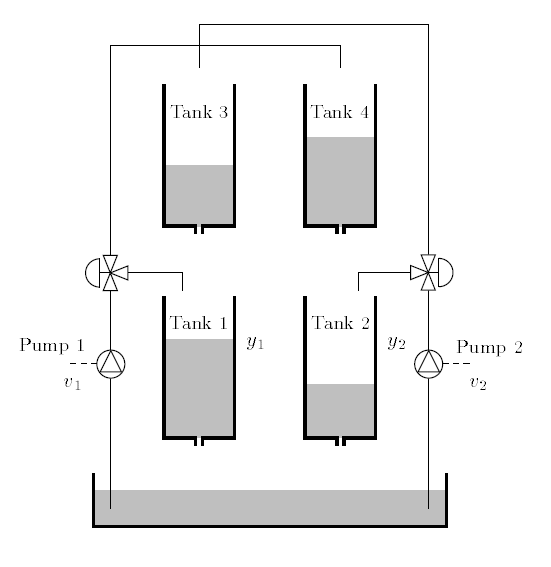
\includegraphics[width=0.5\textwidth]{img/4tank.png}
	\caption{\label{figDesc4tank}Diagrama esquemático do sistema de quatro tanques e planta didática.}
\end{figure}

As bombas impulsionam o fluído do reservatório para o sistemas: bomba 1 para os tanques 1 e 4, bomba 2 para os tanques 2 e 3.  As válvulas definem a proporção direcionada entre os tanques inferior e superior de cada rota.

A \hyperref[imgPlanta]{Imagem \ref{imgPlanta}} a seguir apresenta a planta utilizada neste experimento, localizada no LARA (Laboratório de Automação e Robótica) - SG-11 (UnB) .

\begin{figure}[H]
	\centering
	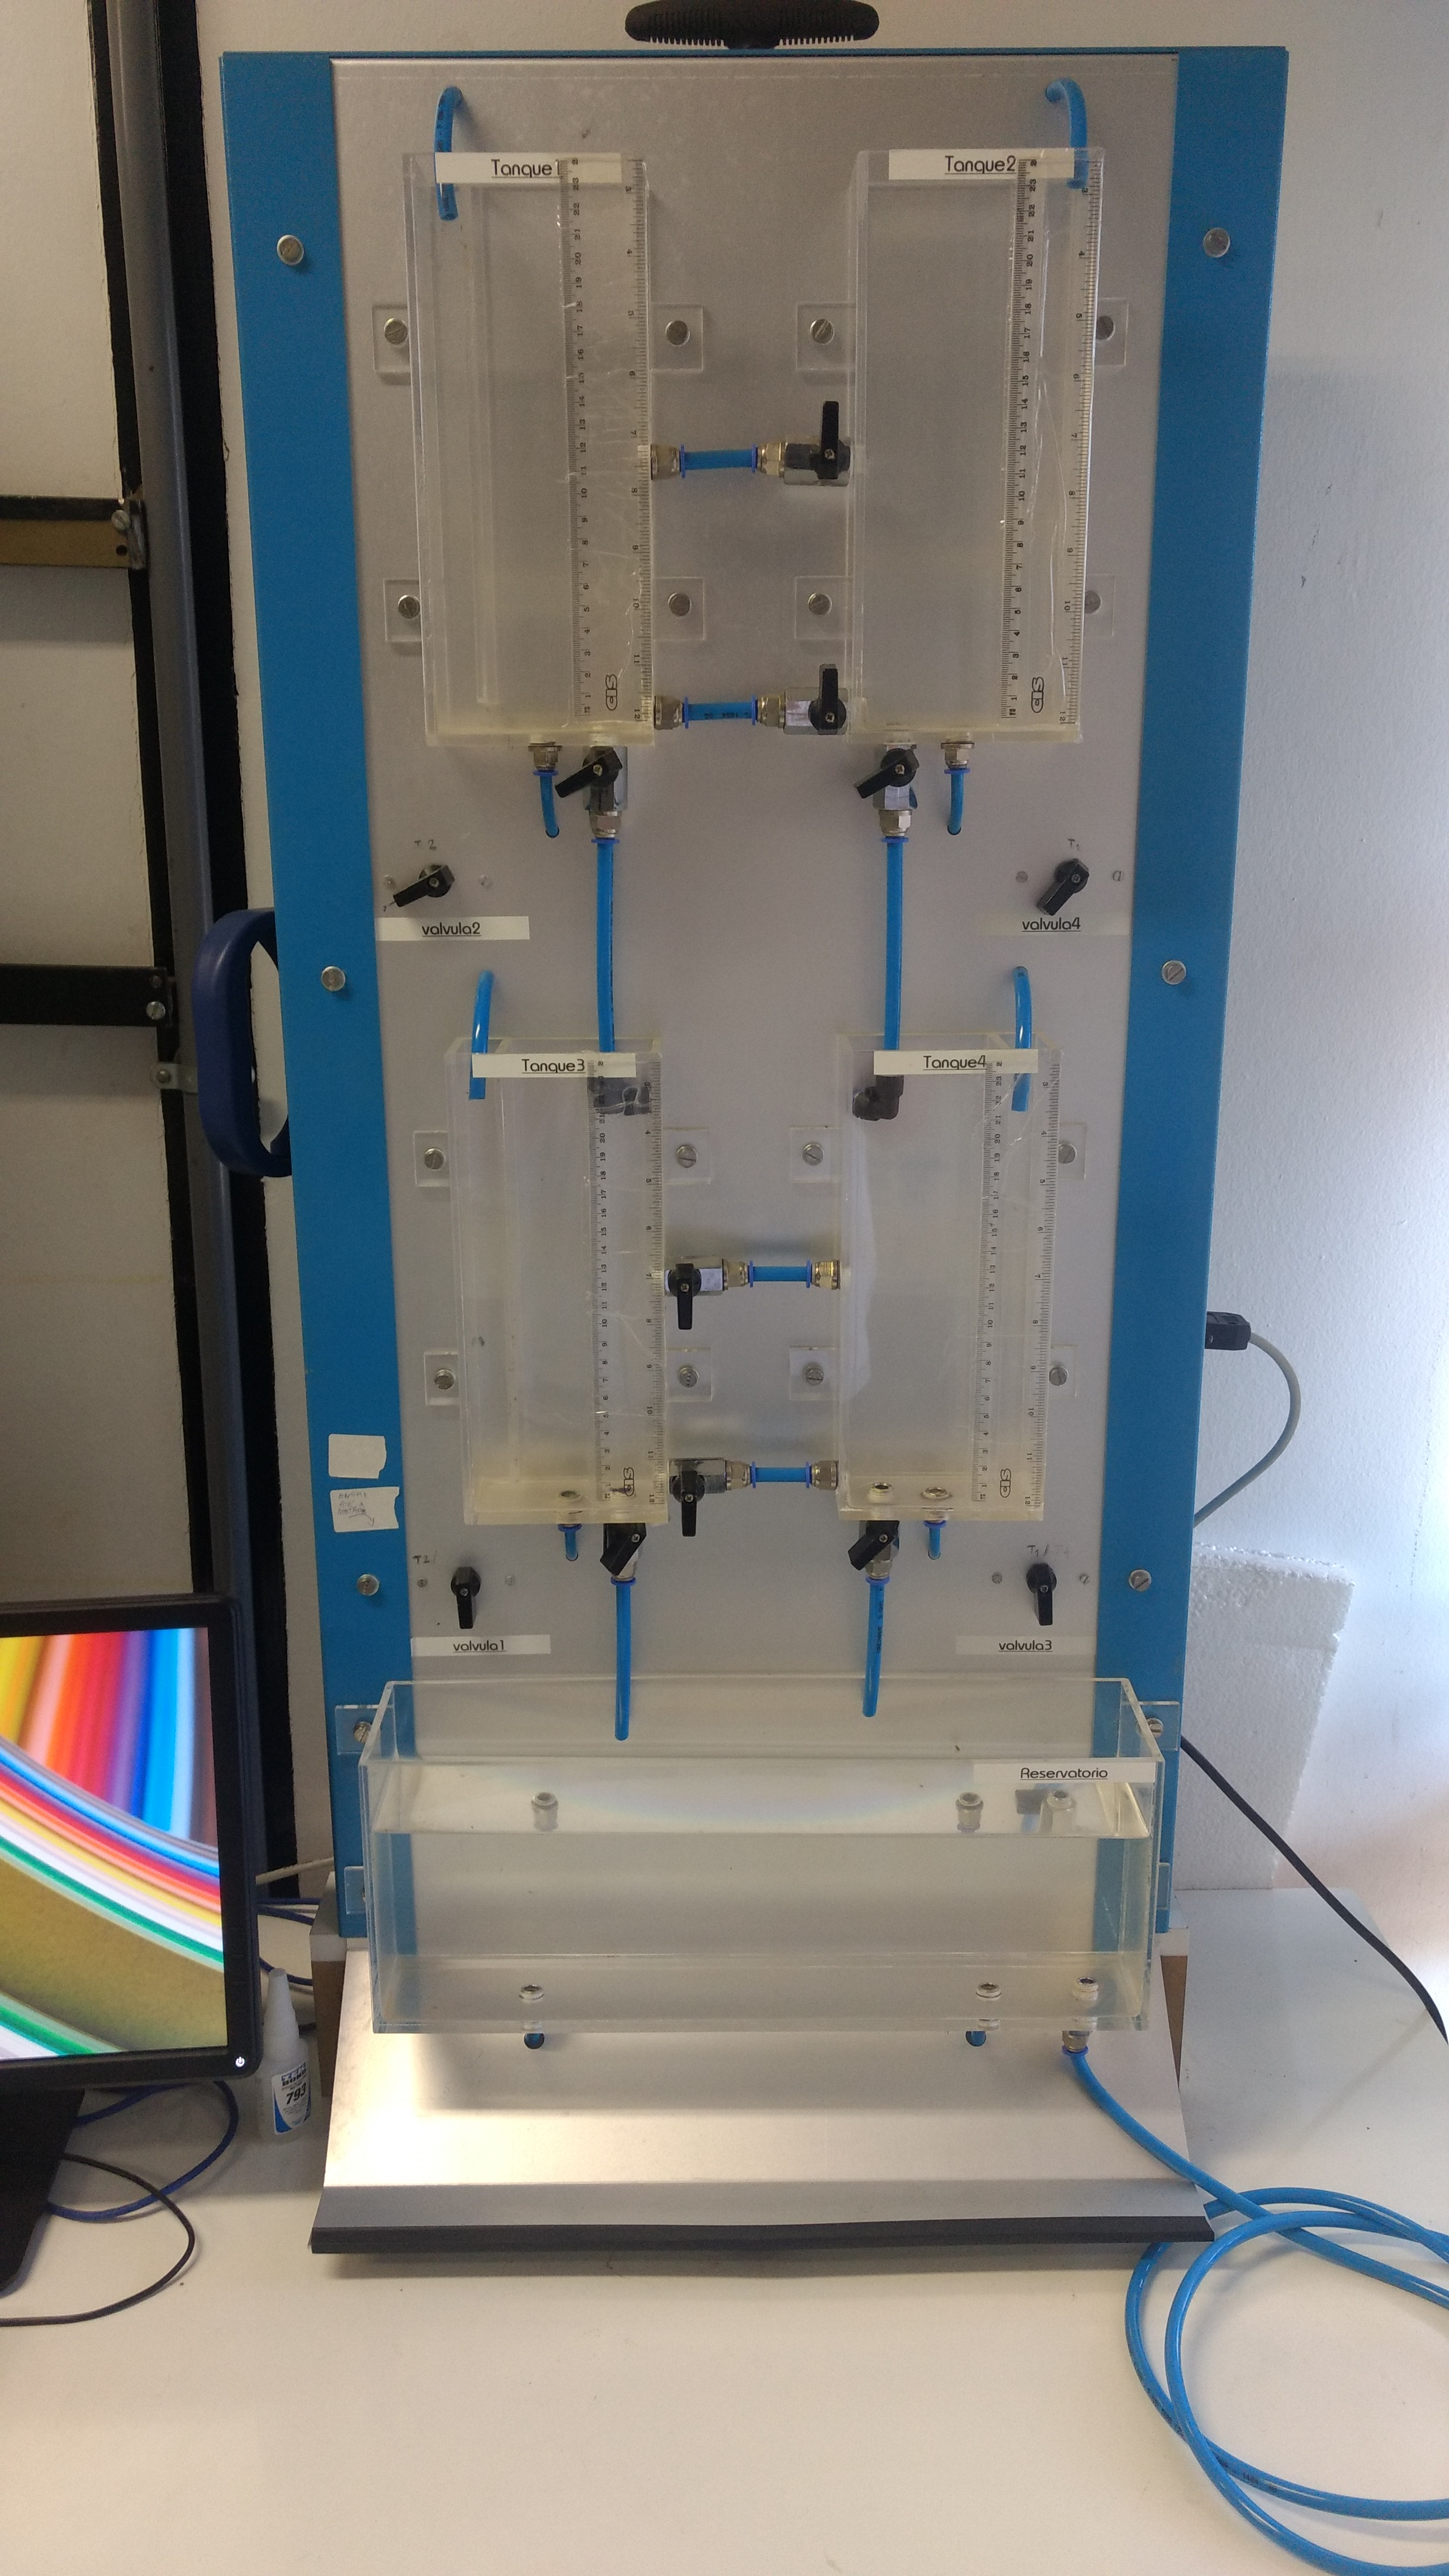
\includegraphics[width=0.4\textwidth]{img/tanqLara.jpg}
	\caption{\label{imgPlanta}Planta de Quatro-Tanques no LARA.}
\end{figure}

Suas dimensões aferidas são apresentadas na \jhhref{tabDescPlanta}{Tabela}, onde $A_{i}$ e $H_{i}$ representam a área da secção transversal da base do tanque e  o nível máximo do tanque $i$, $i = 1,2,3,4$.

\begin{table}[!ht]
	\caption{Especificações Iniciais da Planta.}
	\label{tabDescPlanta}
	\small
	\centering
	\scalebox{1}{
		\begin{tabular}{|c|c|}
			\hline
			\multicolumn{2}{|c|}{Especificações Iniciais da Planta} \\
			\hline
			$A_1$, $A_3$ & 47,6 cm$^2$ \\ \hline
			$A_2$, $A_4$ & 47,6 cm$^2$\\ \hline
			$H_1$, $H_2$, $H_3$, $H_4$ & 24 cm\\ \hline
			$g$ & 981 cm/s$^2$
		\end{tabular}
	}
\end{table}

\section{CLP Rockwell 1756-L62}
Controladores Lógico Programáveis (CLP) são largamente utilizados para controle de processos e automação industrial atualmente. Trata-se de um equipamento eletrônico digital com hardware e software adaptados para as condições industriais. Utilizam uma memória programável para armazenar instruções de controle e conexões com diversos módulos para interface com processos externos, entrada e saída de dados, comunicação digital, entre diversas outras funções.

\subsection{Instalação}
Neste trabalho realizou-se a montagem de toda a estação de controle. Assim, escolheu-se primeiramente um local adequado para a disposição do painel de controle: próximo à planta e ao microcomputador ao qual se conecta, porém afastado de fiações elétricas ou locais úmidos. Outro cuidado deve de ser observado durante a instalação da fonte junto ao chassi, observando a compatibilidade com as tensões de entrada e saída do controlador. Seguiu-se fixação do painel no local escolhida, instalação do microcomputador à ser utilizado e instalação da fiação elétrica. Observa-se na Figura \ref{fig:mesa} o resultado instalado.

\begin{figure}[H]
	\centering
	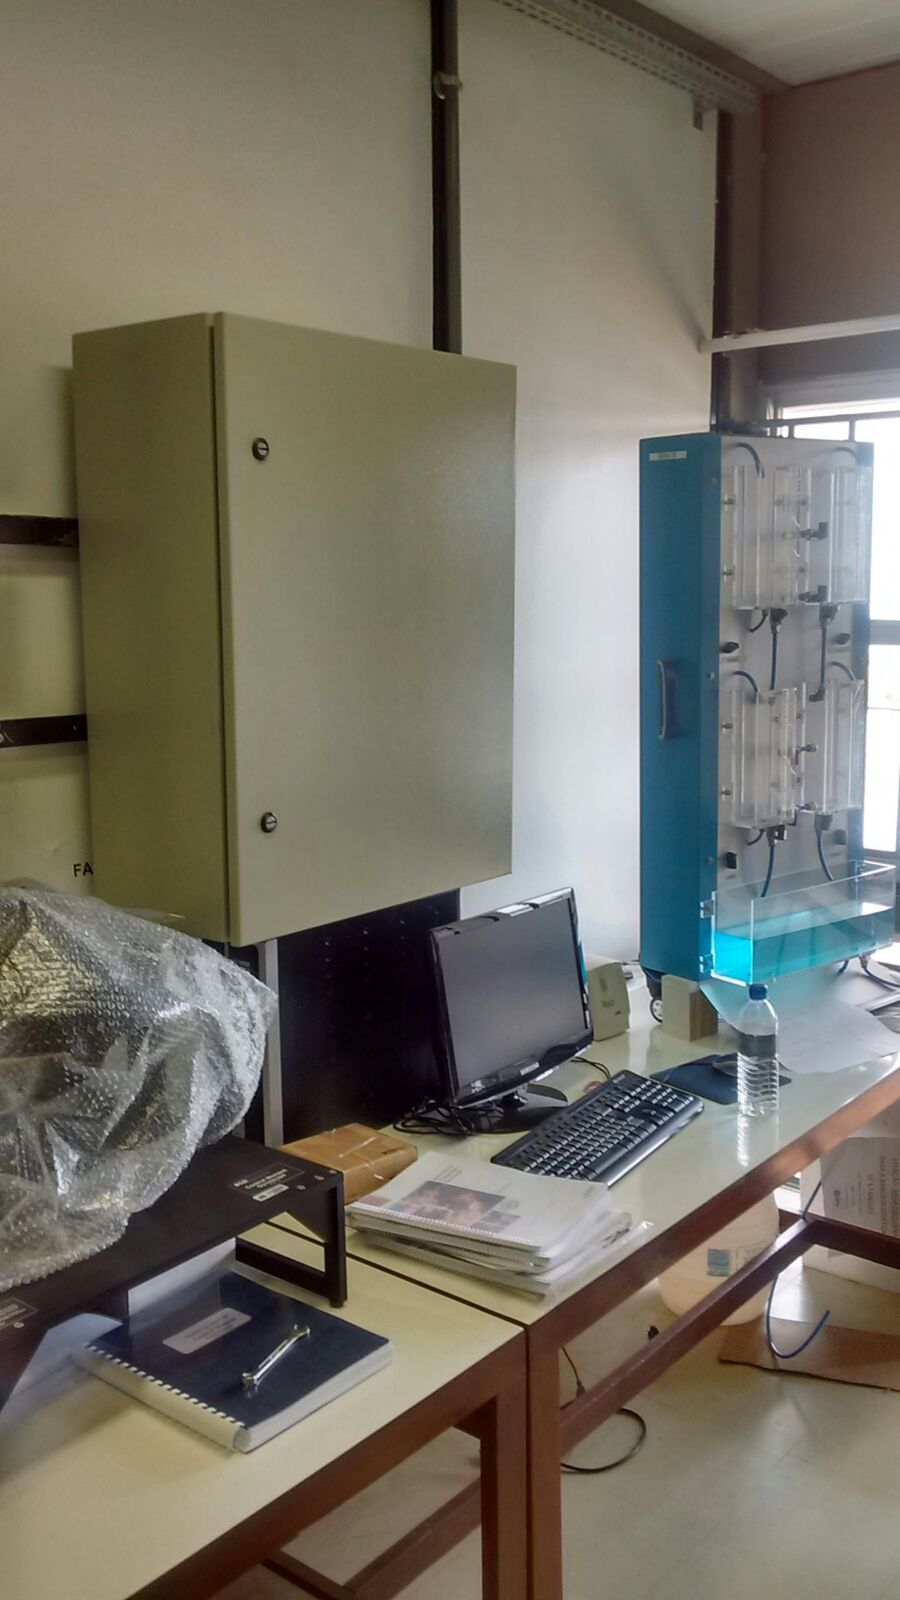
\includegraphics[height=10cm,keepaspectratio]{figs/mesa.jpg}
	\caption{Estação de trabalho.}
	\label{fig:mesa}
\end{figure}

A Figura \ref{fig:interior} a seguir ilustra o interior do painel, já com o chassi do controlador instalado e as trilhas utilizadas distribuídas no espaço restante para conexão dos bornes a serem utilizados no projeto.

\begin{figure}[H]
	\centering
	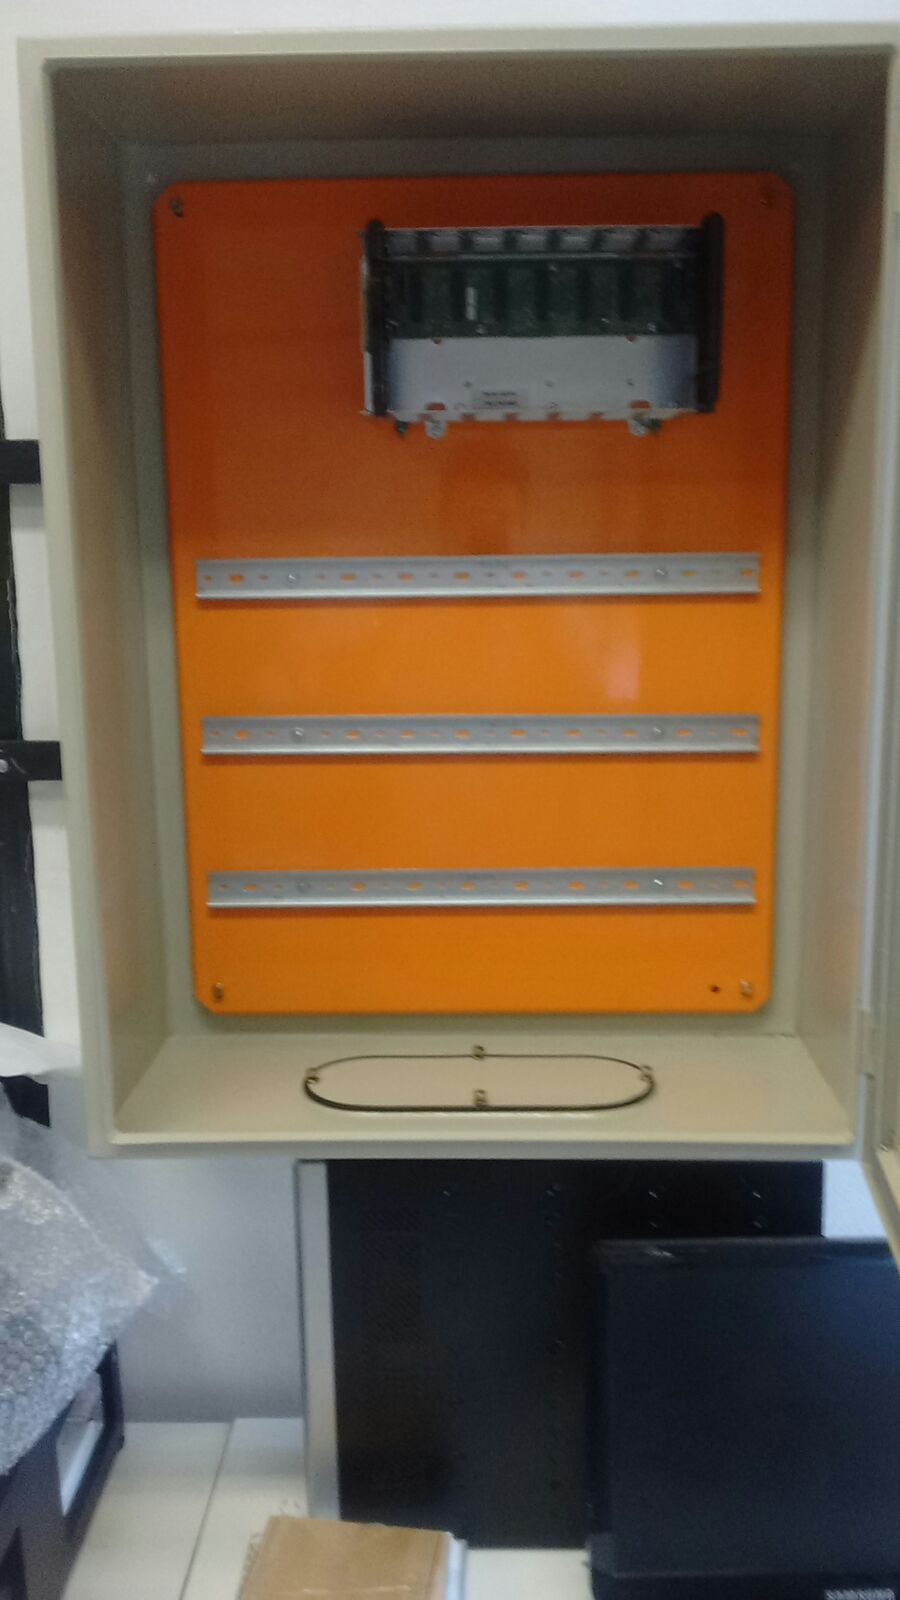
\includegraphics[height=10cm,keepaspectratio]{figs/interior.jpg}
	\caption{Interior do painel.}
	\label{fig:interior}
\end{figure}

Os módulos de entrada e saída foram instalados conforme a \hyperref[tab:modulos]{Tabela \ref{tab:modulos}} abaixo. 

\begin{table}[!ht]
	\caption{Módulos 1756 instalados.}
	\label{tab:modulos}
	\small
	\centering
	\scalebox{1}{
		\begin{tabular}{|c|c|c|}
			\hline
			Especificação & Descrição & Posição no chassi\\
			\hline
			1756-A7/B & Chassi & .\\
			\hline
			1756-L62 & Controlador & 0 \\
			\hline
			1756-ENBT/A & EtherNetIp & 1\\
			\hline
			1756-IF8/A & Entradas Analógicas & 2\\
			\hline
			1756-OF8/A & Saídas Analógicas & 3\\
			\hline
			1756-IB16/A & Entradas DC & 4 \\
			\hline
			1756-OB8I/A & Saídas DC & 5 \\
			\hline
		\end{tabular}
	}
\end{table}

Observa-se na Figura \ref{fig:modulos} a seguir a configuração instalada.

\begin{figure}[H]
	\centering
	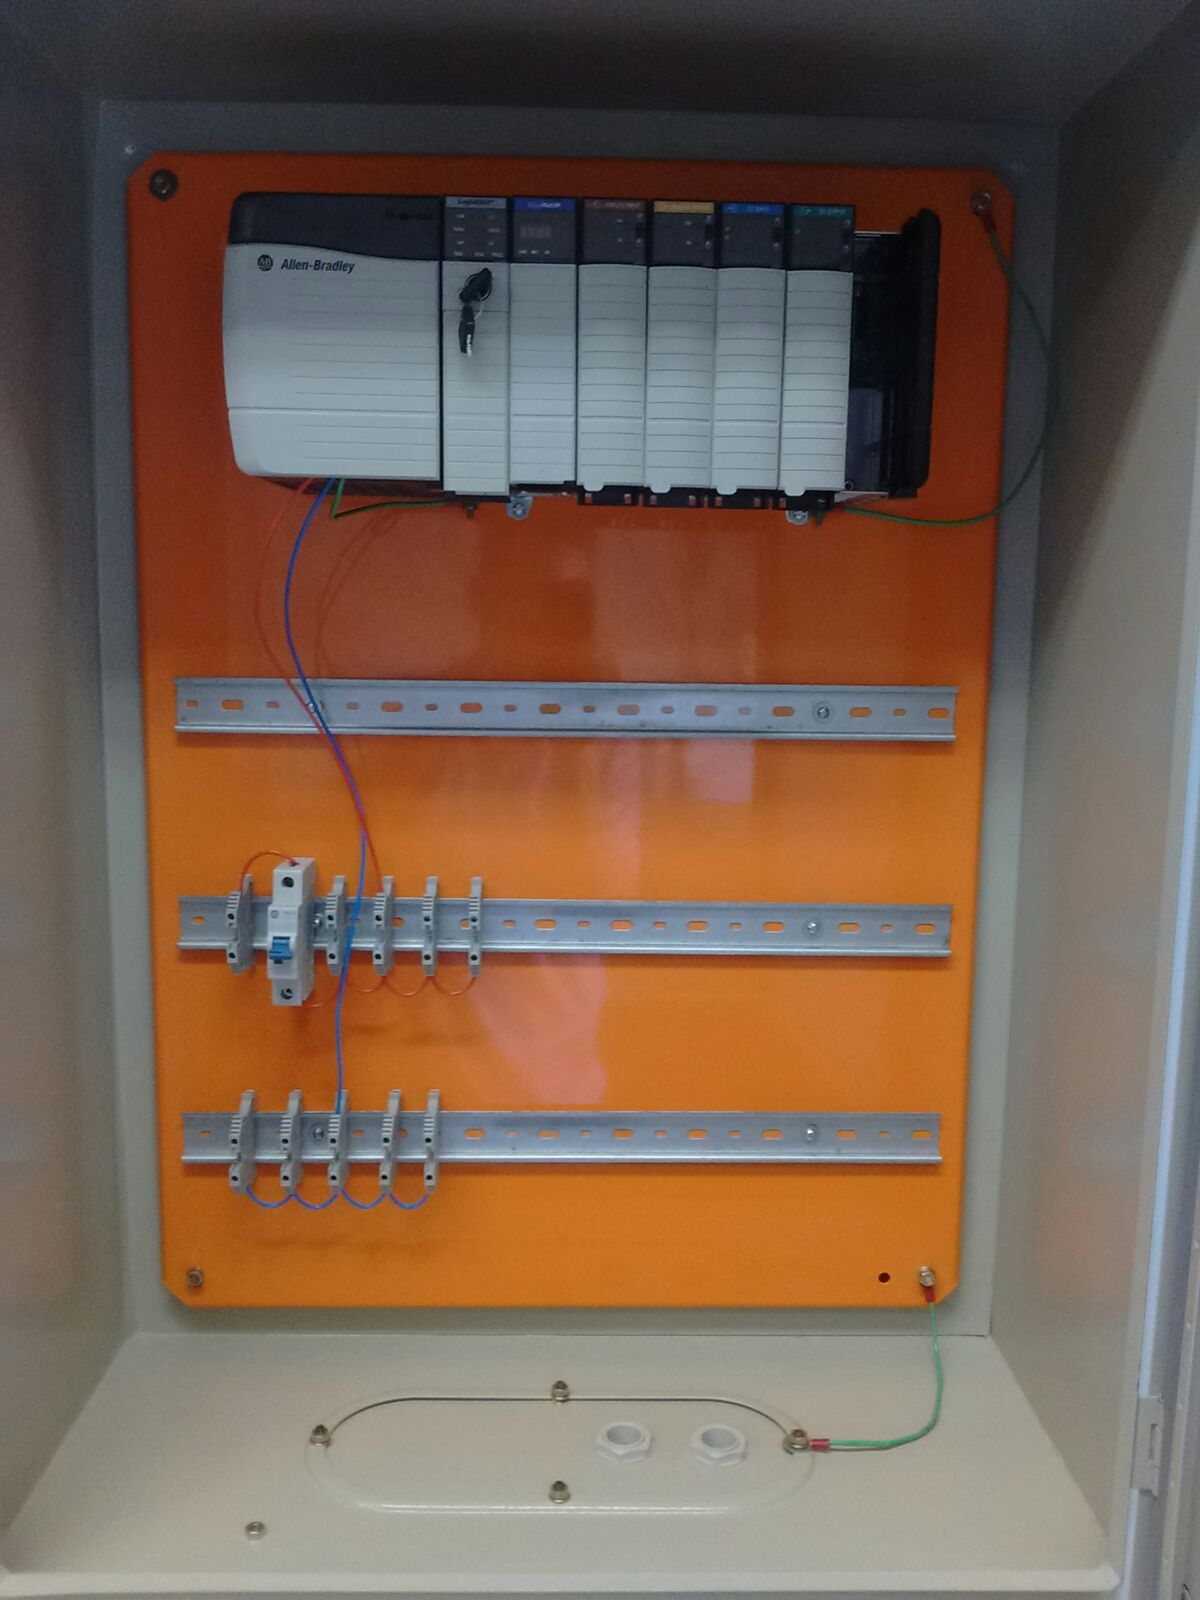
\includegraphics[height=10cm,keepaspectratio]{figs/modulos.jpg}
	\caption{Módulos do painel.}
	\label{fig:modulos}
\end{figure}

\subsection{Integração}
Seguiu-se a configuração dos módulos de comunicação com o CLP. Dois modos são disponíveis com os módulos utilizados: serial, realizada diretamente com o controlador, e Ethernet, através do módulo EtherNetIP. Ambas foram implementadas e testadas.

Para comunicação serial, basta configurar a entrada serial no computador a ser utilizado e em seguida configurar o controlador no software RSLinx \cite{rslinx}. Para utilizar a comunicação EtherNetIp é necessário antes configurar o módulo EhterNetIp \cite{ethernetmodule}. O software BOOTP/DHCP torna possível assinar um endereço IP para o módulo recém instalado. Para que a comunicação em uma rede EtherNetIp ocorra corretamente todos os dispositivos dela precisam possuir endereços IP seguindo o padrão definido pela máscara de sub-rede, neste caso, 255.255.255.0. Isso significa, basicamente, que os pontos comunicantes da rede devem possuir ids únicos apenas nos último octeto de seus endereços. A tabela a seguir apresenta os endereços utilizados, bem como a configuração padrão da rede.

\begin{table}[!ht]
	\caption{IPs dos dispositivos}
	\label{tabIPs}
	\small
	\centering
	\scalebox{1}{
		\begin{tabular}{|c|c|}
			\hline
			\textbf{Dispositivo} & \textbf{Endereço}\\
			\hline
			PC (RSLinx) & 192.168.2.1\\
			\hline
			1756-ENBT/A (CLP) & 192.168.2.22 \\
			\hline
			Geral & 192.168.2.xxx\\
			\hline
		\end{tabular}
	}
\end{table}

Um \textbf{importante} cuidado de segurança observado foi o aterramento de diversos elementos do equipamento. É conhecida sua capacidade de operação em condições adversas, mesmo assim, como precaução houve o cuidado de aterrar o chassi, a placa onde foi instalado e o painel exterior.

\section{RSLinx e RSLogix}
Os principais softwares utilizados para implementação do controlador são o RSLinx e o RSLogix. O primeiro é responsável por estabelecer a comunicação com o CLP Rockwell e sua ampla variedade de aplicativos e módulos. A \jhhref{imgRSLinx}{Figura} apresenta sua interface, onde é possível visualizar o controlador e os módulos instalados. A partir deste menu são acessíveis diversas funções de configuração e exibição das informações dos dispositivos.

\begin{figure}[H]
	\centering
	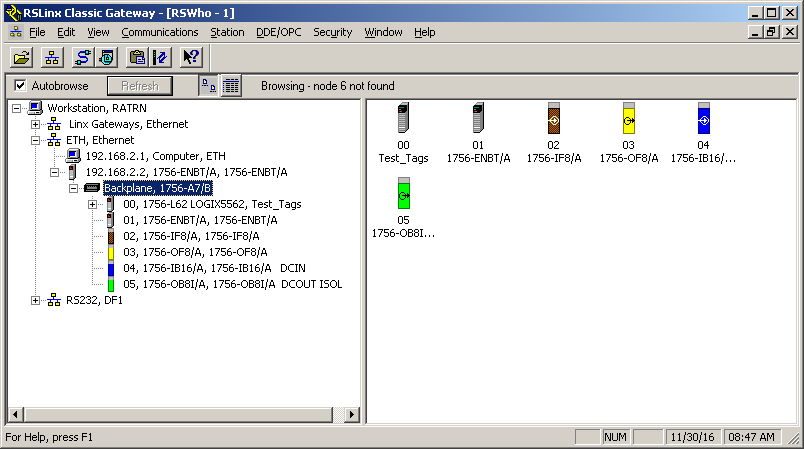
\includegraphics[height=5cm,keepaspectratio]{img/RSLinx.png}
	\caption{Interface do Software RSLinx.}
	\label{imgRSLinx}
\end{figure}

Já o RSLogix 5000 é o ambiente de desenvolvimento proprietário da Rockwell (Allen-Bradley). Neste trabalho, os controladores foram desenvolvidos no RSLogix e enviados (Download) para o CLP em conjunto com o RSLinx. As seções a seguir apresentam as linguagens de o desenvolvimento disponibilizadas pelo RSLogix, a saber linguagem Ladder, blocos de funções e texto estruturado.

\subsection{Linguagem Ladder} \label{subsec:ladder}
A linguagem Ladder é a pioneira dos CLPs por se tratar de uma evolução natural de diagramas elétricos, utilizados antes da chegada dos controladores digitais.  Seu ambiente de desenvolvimento utiliza o posicionamento de de símbolos e blocos para implementação da lógica de controle. 
O ambiente inicial é formado por duas linhas verticais, que representam nível lógico alto (à esquerda) e baixo(à direita) de um sistema. Entre essa linhas são desenhados ramais horizontais que representam representados os estados do CLP.

Uma forma de compreender essa linguagem seria como uma série de conexões de contatos e bobinas. Se for possível traçar um caminho da esquerda para direita, conectando-se à uma bobina de saída ao final, então o valor dessa bobina será verdadeiro. Trabalhando-se com controladores digitais, são criadas variáveis no programa que representam diretamente os valores presentes nos módulos de saída e entrada. Essas variáveis recebem o nome de TAGs. Assim, as variáveis de entradas são assinaladas à tags utilizadas como chaves e as variáveis de saídas à tags associadas às bobinas de saída. Percorrendo-se o caminho da esquerda para direita em um ramal, ao se chegar à uma chave, observa-se se o valor assinalado à ela é verdadeiro. Caso seja, continua-se o caminho até uma bobina de saída. Se está for alcançada, seu valor é setado para verdadeiro, consequentemente a saída associada a ela recebe a tensão associado à este nível lógico no controlador.

A Figura \ref{fig:ladder} à seguir ilustra um exemplo.

\begin{figure}[H]
	\centering
	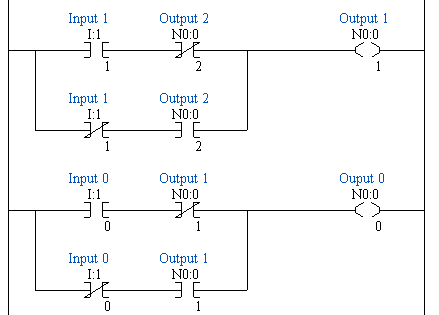
\includegraphics[height=5cm,keepaspectratio]{figs/ladder.png}
	\caption{Exemplo de Diagrama Ladder.}
	\label{fig:ladder}
\end{figure}

\subsection{Blocos Funcionais} \label{subsec:blocos}
Trata-se de outra linguagem de programação gráfica disponível aos CLPs Rockwell. É bastante semelhante à observada em vários outros softwares comuns ao meio acadêmico, como o MATLAB. Para sua utilização, assinala-se tags às entradas e saídas dos módulos já adicionados ao projeto. O desenvolvimento utiliza blocos de entradas e saídas associados à essas variáveis. Conexões entre os blocos, por meio de linhas representam passagem dos valores por esses fios. A lógica de controle é feita por meio de blocos de funções, estes possuem uma ou mais entradas e uma ou mais saídas. Os valores assinalados à suas saídas são determinados pelas funções às quais estão associados e que utilizam os valores de entrada como argumentos.

A Figura \ref{fig:blocos} à seguir ilustra um exemplo.

\begin{figure}[H]
	\centering
	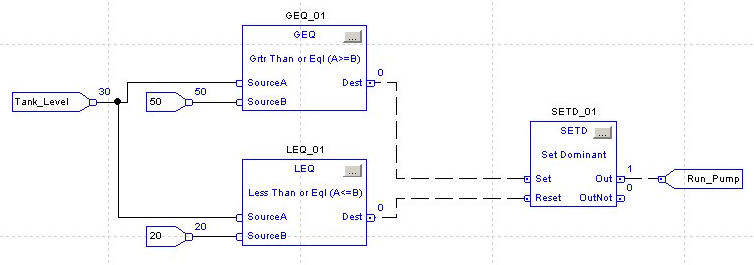
\includegraphics[height=5cm,keepaspectratio]{figs/blocos.png}
	\caption{Exemplo de diagrama de blocos.}
	\label{fig:blocos}
\end{figure}

Observa-se o caso do bloco GEQ\_01. Suas entradas são o nível do tanque (SourceA = Tank\_Level) e um valor constante (SourceB = 50). Sua saída (dest) será assinalada com nível lógico verdadeiro apenas quando $SourceA \geq SourceB$, ou seja, $Dest=1$ se $Tank\_Level \geq 50$, sendo $Dest = 0$ caso contrário.

\subsection{Texto Estruturado} \label{secTexEst} 
A linguagem texto estruturado é muito semelhante às linguagens estruturais C e Pascal. Como elas, é baseada no uso simples de comandos que são executados sequencialmente em seu desenvolvimento. Da mesma forma que as anteriores, esta linguagem utiliza Tags como variáveis e é a partir delas que se faz a leitura das entradas e definem-se as saídas. 

A \jhhref{imgTexEst}{Figura} à seguir ilustra um exemplo.

\begin{figure}[H]
	\centering
	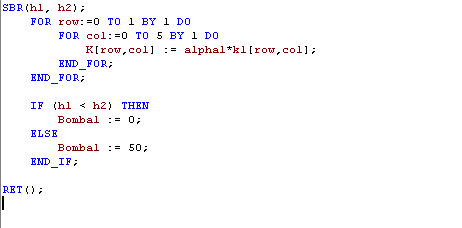
\includegraphics[height=5cm,keepaspectratio]{img/strText.png}
	\caption{Exemplo de Texto Estruturado.}
	\label{imgTexEst}
\end{figure}

%% TODO: Exemplo
\selectlanguage{brazil}%



\selectlanguage{english}%

\chapter{Título do Capítulo}

Lorem ipsum dolor sit amet, consectetur adipiscing elit. Sed elementum
gravida risus non accumsan. Vivamus est magna, rhoncus a aliquam ut,
faucibus vitae ligula. Nam rhoncus dolor nec erat rhoncus eu sagittis
turpis ultrices. Quisque nisl neque, dictum ut congue eget, pellentesque
in felis. Pellentesque iaculis, quam eget rhoncus ultrices, augue
turpis malesuada ligula, nec dignissim metus lacus sed ligula. Duis
imperdiet risus eget nulla dictum non condimentum neque vestibulum.
Integer fringilla, nisl et viverra laoreet, arcu ante malesuada lorem,
vel ullamcorper odio orci eget eros. Maecenas hendrerit nisl in nibh
viverra sed dignissim ante sagittis. Nullam dignissim faucibus felis,
non interdum mi lacinia id. Pellentesque in sapien in sem malesuada
consectetur. Vivamus nec lacus et odio rhoncus cursus. Aliquam condimentum
purus sit amet purus adipiscing tempor non sed ipsum. Aenean vestibulum
sodales risus, ac rutrum dui molestie pharetra. 

\section{Introdução}

Mauris viverra orci sit amet \cite{article:dummy} mi varius at porta
felis volutpat. Aenean pharetra ultricies justo quis ultricies. Etiam
posuere gravida egestas. Nullam ac tortor in mi porta rutrum ac ac
tortor. Curabitur elit purus, cursus quis elementum tincidunt, facilisis
sit amet leo. Nam adipiscing eleifend ipsum, in viverra lorem luctus
rutrum. Donec vitae velit eros. Pellentesque habitant morbi tristique
senectus et netus et malesuada fames ac turpis egestas. Aliquam semper,
magna sed pulvinar blandit, sem ante eleifend nibh, et ultrices nisl
magna a urna. In fringilla, sapien aliquam dapibus vestibulum, nunc
orci commodo ipsum, vel rutrum tortor nulla vel mauris.

Lorem ipsum dolor sit amet, consectetur adipiscing elit. Etiam cursus
laoreet turpis, ac hendrerit ipsum gravida non. Vestibulum imperdiet
mattis quam, sed interdum purus placerat eu. Sed eget lectus sed justo
scelerisque placerat. Ut luctus purus viverra nulla tincidunt vitae
fermentum tortor pellentesque. Pellentesque eleifend sagittis ipsum
eu sagittis. Integer ultricies adipiscing sem, a lacinia sapien pharetra
sed. Sed consectetur orci at odio aliquet in placerat libero lobortis.
Vestibulum ullamcorper nibh ligula, nec dictum leo. Maecenas consectetur
tristique risus sit amet auctor. Maecenas ultrices sodales convallis.
Mauris ut leo ut purus sodales blandit molestie sed lectus. In hac
habitasse platea dictumst. In ultrices pharetra lacus, a posuere tellus
sagittis malesuada. Etiam consectetur laoreet diam, a iaculis turpis
porttitor nec.

Vivamus in nisl magna. Vestibulum odio metus, consequat sed mollis
in, consectetur id enim. Donec nec odio turpis, a convallis quam.
Phasellus vitae felis porttitor risus molestie imperdiet. Class aptent
taciti sociosqu ad litora torquent per conubia nostra, per inceptos
himenaeos. Integer non velit lacus, vitae iaculis nunc. Curabitur
diam mi, aliquet nec vehicula faucibus, gravida eu nisi.

Aliquam erat volutpat. Nam ligula arcu, ultricies sit amet tempor
ut, consectetur non metus. Class aptent taciti sociosqu ad litora
torquent per conubia nostra, per inceptos himenaeos. Integer semper
dictum sapien, et fringilla est interdum eget. Morbi posuere augue
ut justo dictum ullamcorper. Quisque non orci metus, non rhoncus erat.
Ut nec sem mi. Curabitur dolor sem, luctus ac cursus at, sollicitudin
id turpis. Nulla scelerisque convallis ante, eget tristique ligula
dictum non. Curabitur dictum, lorem in adipiscing rhoncus, justo nibh
placerat augue, eu molestie enim justo non tortor. Quisque odio risus,
egestas vel dapibus in, rutrum vitae turpis. Curabitur adipiscing
lectus at purus imperdiet malesuada consequat nibh viverra. Morbi
in nisi porttitor massa dapibus facilisis. Phasellus consectetur arcu
non massa ultrices aliquam.

Nullam ut sapien semper neque tempor imperdiet. Vivamus vel congue
nulla. Mauris posuere blandit suscipit. In feugiat lobortis vehicula.
Maecenas vel magna vel turpis sollicitudin aliquet. Phasellus neque
dui, egestas id vulputate id, facilisis eu nibh. In hac habitasse
platea dictumst. Aliquam et dolor turpis, vel mollis lacus. Nunc in
nisl at lectus rutrum ullamcorper. Nullam venenatis nisl in velit
rutrum quis semper mauris facilisis. Proin sollicitudin, eros sit
amet bibendum ornare, dui risus mattis dui, et elementum nisi turpis
id sapien.

Proin sollicitudin, nisl at pellentesque tempus, arcu erat viverra
odio, sed feugiat enim mi posuere leo. Proin orci nisi, dignissim
et pharetra at, ultrices in felis. Quisque leo libero, tristique vitae
varius eget, sodales vitae ante. Vestibulum placerat mauris vitae
augue feugiat ultricies. Quisque rutrum dui eu nibh volutpat auctor.
Aenean vulputate accumsan eros ac fermentum. In hac habitasse platea
dictumst. Fusce vestibulum ante quis sem vestibulum vehicula. Morbi
neque augue, interdum eget cursus id, ullamcorper et purus. Maecenas
pretium sagittis mauris eget condimentum. Sed sodales facilisis dignissim.
Cras quis gravida turpis. Nullam mattis gravida commodo. Nulla et
est at enim commodo imperdiet.

Vestibulum ante ipsum primis in faucibus orci luctus et ultrices posuere
cubilia Curae; Cras eros magna, tempus a aliquet ut, consectetur non
quam. Morbi a turpis nisl, sit amet sodales ante. Sed et pretium elit.
Nam elementum leo at diam porttitor sit amet ullamcorper dolor egestas.
Vestibulum ante ipsum primis in faucibus orci luctus et ultrices posuere
cubilia Curae; Cum sociis natoque penatibus et magnis dis parturient
montes, nascetur ridiculus mus.

Cras non tellus eu tortor tincidunt semper at vel nibh. Quisque felis
justo, sodales non semper eu, lacinia et massa. Aliquam id dui odio,
et mattis dui. Donec tempus, nulla a porta adipiscing, purus nunc
convallis nunc, sit amet consectetur mi eros aliquet mauris. Ut et
velit in leo sagittis tincidunt. Mauris non varius dolor. Etiam ac
nibh felis. Donec pulvinar porta nisl, a sollicitudin eros pellentesque
a. Duis scelerisque mi in libero convallis sed condimentum libero
aliquam.

Vivamus suscipit orci a justo tempus ultrices. Proin volutpat magna
a purus condimentum non malesuada diam tristique. Pellentesque nibh
enim, posuere accumsan rhoncus mollis, dignissim ut quam. Nullam eget
tempus ante. Proin dignissim suscipit lacus eget venenatis. Quisque
sollicitudin mi at orci lobortis ac semper urna interdum. Aenean at
est eget tellus porta laoreet. Aliquam et quam et risus vulputate
luctus et a metus.

Praesent velit mauris, venenatis sed aliquam at, fermentum in augue.
Etiam dictum, eros ut posuere feugiat, tellus risus hendrerit ipsum,
quis aliquet eros risus at erat. Duis commodo auctor gravida. Proin
accumsan nibh id eros molestie vel fermentum diam iaculis. Nulla venenatis
tincidunt hendrerit. Morbi ultricies, felis sed elementum aliquam,
lectus turpis rutrum risus, ut rhoncus orci urna eu sapien. Aenean
commodo tortor ipsum. Vivamus eros nibh, varius ac mattis id, interdum
ac felis. Aliquam laoreet mi at metus congue pharetra. Proin et tortor
sed mauris bibendum commodo quis commodo tellus.

Mauris augue nibh, eleifend nec fringilla non, tristique at arcu.
Praesent sagittis, massa vitae consectetur rhoncus, justo erat volutpat
leo, sit amet ultrices enim lectus sed mauris. Mauris a massa et lectus
feugiat rutrum ac eu lectus. Maecenas et enim purus, et faucibus lorem.
Pellentesque vel sagittis lacus. Integer nec libero magna. Suspendisse
vulputate sapien sit amet nibh porta in accumsan nisl gravida. Donec
tempus molestie diam, vel sollicitudin lacus interdum non. Vivamus
tellus erat, cursus nec iaculis eu, porta at nisl. Nullam fermentum
tincidunt metus, ac bibendum ligula gravida sed. Donec vitae ante
in sem commodo posuere ac vitae mauris.

Curabitur aliquam ultricies nunc, a vulputate nisl rhoncus id. Sed
sagittis lectus nec lacus tincidunt hendrerit. Etiam egestas aliquet
nibh, eget pretium lorem mollis non. Quisque porttitor imperdiet erat
at varius. Praesent a leo mi. Maecenas quam tellus, aliquet id porta
a, luctus nec metus. Donec facilisis enim in massa sagittis nec sollicitudin
sem dapibus. Suspendisse iaculis, nibh non porta porta, lacus tortor
suscipit nunc, eget sagittis felis urna at dolor. Cras luctus hendrerit
justo, non hendrerit nisi lacinia nec. Duis in erat nisi. Maecenas
at libero dolor. Aenean vel nulla quis tortor lobortis iaculis. Sed
tempor, arcu sit amet bibendum hendrerit, dolor urna convallis ligula,
quis volutpat lorem purus nec nisl. Sed eros augue, pulvinar eu posuere
consectetur, aliquam a tellus. Vestibulum lorem leo, condimentum a
cursus sit amet, lobortis ac magna. Mauris in orci quis lorem mollis
pellentesque.

Donec blandit volutpat erat et ultricies. Integer mattis porta dolor
porta porta. Nulla mauris urna, vestibulum at semper a, porta ac magna.
Mauris tempor mi id augue consequat egestas. Vivamus ultricies mi
sed arcu dapibus convallis. Integer ac nibh vitae libero rhoncus sodales
in ut urna. Proin eget leo purus, ac scelerisque arcu. Phasellus cursus
laoreet commodo. Sed at ante enim. Nullam quis ante lacus. Aliquam
eros sapien, interdum non semper ut, facilisis sed ipsum.

Aenean eleifend, arcu at dictum cursus, felis neque dictum orci, at
blandit tellus mi et dui. Donec pretium orci vel justo rutrum viverra.
Pellentesque habitant morbi tristique senectus et netus et malesuada
fames ac turpis egestas. Integer cursus, metus ac venenatis consequat,
lectus risus sollicitudin odio, iaculis dictum nisi quam vel est.
Fusce pellentesque sagittis varius. Etiam dapibus nisi blandit mi
iaculis aliquet. Suspendisse potenti. Aenean mi urna, feugiat vitae
accumsan et, venenatis in magna. In in sollicitudin ligula.

Phasellus suscipit molestie nisl imperdiet blandit. Aliquam velit
augue, scelerisque tincidunt accumsan vel, cursus et lacus. Vestibulum
non augue a dolor aliquet elementum ut ac mauris. Nulla facilisi.
Cras commodo augue vel nulla scelerisque et accumsan turpis dictum.
Quisque fermentum, metus non aliquam venenatis, urna mi vehicula nulla,
quis molestie dui quam vel ante. In hac habitasse platea dictumst.
Morbi tristique massa sed massa condimentum accumsan. Praesent id
felis eu mauris tincidunt egestas. Sed vulputate, metus quis aliquam
fringilla, metus ligula interdum risus, sit amet tristique quam dui
quis sapien. Phasellus et tortor non sapien vehicula pellentesque.

Nulla facilisi. Cum sociis natoque penatibus et magnis dis parturient
montes, nascetur ridiculus mus. Proin et pretium nulla. Donec at luctus
libero. Maecenas et nisl velit, ut aliquet ante. Vestibulum ac nibh
eget orci facilisis vulputate quis sed arcu. Vestibulum sit amet odio
quam, quis tempus diam. Vivamus nec porta turpis. Curabitur dui orci,
feugiat ac ornare eget, commodo ut justo. Aenean vel tempus ante.

Maecenas auctor velit et augue fermentum sit amet vestibulum enim
dapibus. Aliquam ac velit magna. Praesent sit amet nulla vel libero
ultrices dapibus vitae consectetur justo. Sed eget diam purus, congue
suscipit sapien. Duis elit tellus, aliquet vitae sodales at, malesuada
vel justo. Cum sociis natoque penatibus et magnis dis parturient montes,
nascetur ridiculus mus. Nulla adipiscing, est ac mollis egestas, lectus
quam luctus urna, vel elementum enim massa id quam. Nullam justo elit,
tincidunt ac dignissim sit amet, suscipit eu urna. Sed mollis turpis
id nisi eleifend in sodales felis volutpat. Vestibulum et ipsum ac
felis hendrerit aliquet. Nulla euismod convallis turpis eu porta.
Nullam ac tellus ut nulla venenatis convallis vitae et leo. Donec
semper commodo dolor, eu interdum mauris rutrum sit amet. Fusce ac
velit nunc.

Maecenas nec orci at augue sollicitudin egestas. Suspendisse non risus
eget sapien sagittis ullamcorper ut at dolor. Class aptent taciti
sociosqu ad litora torquent per conubia nostra, per inceptos himenaeos.
Quisque a vestibulum augue. Donec erat mauris, molestie sed sagittis
sed, porttitor id elit. Nunc blandit accumsan lacus eu semper. Aliquam
cursus diam vel massa iaculis vitae laoreet tortor lacinia. Sed nibh
velit, dapibus et lacinia rutrum, rutrum id lorem. Aenean consectetur
accumsan elit, nec cursus dui commodo nec. Integer id elit vel mi
vulputate interdum sit amet sed tortor. Morbi auctor sem nec mauris
blandit eleifend. Aliquam erat volutpat. Donec mattis justo justo,
et condimentum lectus. Praesent suscipit arcu ac nunc pellentesque
consectetur.

Nunc at enim sit amet neque malesuada imperdiet non eget velit. Praesent
pharetra tempor lobortis. Class aptent taciti sociosqu ad litora torquent
per conubia nostra, per inceptos himenaeos. Nunc in massa vel elit
vulputate porttitor. Nulla semper, ipsum nec elementum tempus, sem
metus consequat libero, id ultrices lacus lacus non metus. Curabitur
at risus at est blandit scelerisque vel nec lorem. Quisque risus odio,
feugiat vitae pharetra vel, sollicitudin sed arcu. Morbi semper quam
sed urna consectetur facilisis. Lorem ipsum dolor sit amet, consectetur
adipiscing elit. Maecenas ante arcu, tristique vel blandit id, facilisis
et metus.

Nullam placerat aliquet augue at tincidunt. Maecenas pellentesque
vulputate lectus ut laoreet. Nulla euismod dignissim euismod. Sed
non ipsum et tortor vulputate accumsan sit amet ut odio. Cras interdum
fringilla risus, ut auctor enim imperdiet ut. Mauris dapibus adipiscing
libero vitae gravida. Proin gravida interdum arcu eget porta. Nunc
at pulvinar urna. Mauris ante nulla, laoreet quis pellentesque eget,
auctor nec nunc. Mauris faucibus, tellus a scelerisque facilisis,
nibh mauris vestibulum lacus, quis rhoncus neque mi pretium augue.
Nam tristique arcu auctor mauris sollicitudin nec rutrum dui lacinia.
Morbi euismod dignissim odio, sed vestibulum sem sodales nec. Cras
mollis convallis lorem, nec sollicitudin ipsum sagittis et. Cum sociis
natoque penatibus et magnis dis parturient montes, nascetur ridiculus
mus. Nam sit amet rhoncus risus.

Fusce molestie mi ut justo pellentesque scelerisque. In hac habitasse
platea dictumst. In fringilla erat eu odio pharetra sodales. Sed ac
sapien id justo adipiscing commodo. Lorem ipsum dolor sit amet, consectetur
adipiscing elit. Donec aliquam enim a sem rhoncus ac accumsan tortor
fermentum. Praesent non ligula nisl. Proin ullamcorper augue nec nulla
bibendum at rhoncus augue cursus. Nunc ac bibendum mauris. Nulla non
lacus diam. Praesent tellus enim, elementum at viverra id, dictum
in lacus. Sed nec libero eget felis suscipit dapibus. Proin ultricies
mauris eget velit cursus molestie. Duis at eros vel ligula faucibus
congue vitae nec ligula. Morbi in sodales magna. Suspendisse accumsan
adipiscing nisi, quis interdum leo facilisis eget.

Integer at mi porta velit porttitor posuere. Aliquam erat volutpat.
Donec a lorem erat. Vivamus vitae nulla vitae nulla placerat laoreet.
Mauris ornare, risus id vestibulum rhoncus, turpis orci viverra risus,
vitae aliquam arcu mauris vel nulla. Aliquam diam nisl, volutpat eu
luctus vel, tincidunt at nulla. Vestibulum porttitor consequat nulla,
ut semper mi sollicitudin id. Maecenas eleifend neque sed arcu tincidunt
facilisis. Etiam quis arcu magna. Ut leo dolor, sagittis nec accumsan
vel, imperdiet rutrum libero. Vestibulum ante ipsum primis in faucibus
orci luctus et ultrices posuere cubilia Curae;

Nam suscipit mauris in ipsum hendrerit tincidunt. Ut rutrum fermentum
bibendum. Donec id eros erat, a porta libero. Sed vitae sapien diam.
In lacinia risus eget tellus dapibus interdum. Etiam libero felis,
vehicula quis lacinia eu, vulputate et tellus. Praesent a leo nisi.
In feugiat odio quis tortor consequat sed condimentum dolor tincidunt.
Cras fermentum ipsum at ipsum lobortis id faucibus tellus consectetur.
Donec euismod suscipit porta. Fusce quis mollis ipsum. Vivamus placerat
sodales eros. Integer suscipit ligula non tortor sollicitudin sed
suscipit sem dictum. Morbi consectetur magna at est semper sit amet
ornare quam porta. Praesent porttitor luctus risus sit amet volutpat.
Class aptent taciti sociosqu ad litora torquent per conubia nostra,
per inceptos himenaeos.

Pellentesque at turpis in risus laoreet auctor. Curabitur sed urna
mauris. Aenean eu nibh sem. Ut dictum, risus vitae hendrerit pretium,
lectus sem condimentum nulla, eu imperdiet justo nisl et turpis. Aenean
ut velit in sapien hendrerit convallis. Quisque volutpat mi ut diam
accumsan condimentum. Quisque quis diam tincidunt turpis semper blandit
quis in nisi. Class aptent taciti sociosqu ad litora torquent per
conubia nostra, per inceptos himenaeos.

Nam ac enim sit amet elit euismod venenatis. Nunc ut dui dolor. Cras
scelerisque tellus at lectus malesuada a interdum ipsum commodo. Praesent
nec tincidunt neque. Donec a odio nunc. Praesent gravida sapien tortor,
vitae eleifend dui. Quisque vitae arcu et nulla rutrum accumsan. Sed
vel mauris vitae risus luctus pharetra nec vitae nisi. Cras et est
eget dolor faucibus ullamcorper ut nec lacus. Sed quis diam scelerisque
lacus eleifend luctus.

Class aptent taciti sociosqu ad litora torquent per conubia nostra,
per inceptos himenaeos. Aliquam non velit consequat nibh ultricies
venenatis. Donec massa diam, sollicitudin ac aliquet consequat, sagittis
a lectus. Morbi porta ligula nec lorem placerat eleifend. Donec consequat
gravida pulvinar. Donec sagittis dui vel magna suscipit ornare. Phasellus
dui tortor, feugiat nec laoreet eget, commodo quis magna. Nam dictum
pellentesque mauris ut fringilla. Fusce vel lectus nunc, sed luctus
mi.

Vestibulum metus metus, rhoncus nec vulputate ac, sollicitudin accumsan
elit. Donec ut est lorem, sit amet vehicula lectus. Sed viverra ultrices
fermentum. Nam massa ipsum, elementum vitae fringilla a, blandit id
arcu. Integer a rutrum lectus. Duis aliquam purus eget eros facilisis
imperdiet. Aliquam condimentum scelerisque tempus. Maecenas adipiscing
vulputate lacus nec laoreet. Ut nunc tellus, tincidunt vitae gravida
sed, adipiscing ut massa. Morbi sed lorem nisl, sit amet tempus dolor.
Vestibulum eu diam eu justo mollis laoreet vel eleifend odio.

Vestibulum commodo nulla quis orci tempus egestas. Aenean elementum
rutrum magna ac tincidunt. Nunc viverra volutpat sem non aliquam.
Lorem ipsum dolor sit amet, consectetur adipiscing elit. Mauris sit
amet tellus justo. Suspendisse placerat faucibus arcu eu lacinia.
Duis blandit massa sollicitudin neque dignissim varius. Donec lacus
lectus, imperdiet sit amet feugiat sit amet, consequat a nibh. Sed
non justo metus, auctor malesuada est.

Integer a nibh elit. Etiam suscipit, lectus vitae aliquet vehicula,
est orci vulputate mauris, eu faucibus tortor metus quis lectus. Aenean
at venenatis dolor. Mauris sodales enim quis nisi mattis a adipiscing
orci semper. Phasellus accumsan tristique metus, in scelerisque nisi
lacinia cursus. Suspendisse potenti. Nam vitae lacus condimentum justo
adipiscing semper at nec metus. Suspendisse placerat suscipit congue. 

\section{Contextualização}

Maecenas nec orci at augue sollicitudin egestas. Suspendisse non risus
eget sapien sagittis ullamcorper ut at dolor. Class aptent taciti
sociosqu ad litora torquent per conubia nostra, per inceptos himenaeos.
Quisque a vestibulum augue. Donec erat mauris, molestie sed sagittis
sed, porttitor id elit. Nunc blandit accumsan lacus eu semper. Aliquam
cursus diam vel massa iaculis vitae laoreet tortor lacinia. Sed nibh
velit, dapibus et lacinia rutrum, rutrum id lorem. Aenean consectetur
accumsan elit, nec cursus dui commodo nec. Integer id elit vel mi
vulputate interdum sit amet sed tortor. Morbi auctor sem nec mauris
blandit eleifend. Aliquam erat volutpat. Donec mattis justo justo,
et condimentum lectus. Praesent suscipit arcu ac nunc pellentesque
consectetur.

\begin{figure}
\begin{centering}
\subfloat[\label{fig:Fig-1}Fig 1]{\begin{centering}

\includegraphics[width=3cm]{figs/chapt02/lara_logo}
\par\end{centering}
} \qquad{} \subfloat[Fig 2]{\begin{centering}

\includegraphics[width=3cm]{figs/chapt02/lara_logo}
\par\end{centering}
}
\par\end{centering}
\caption{\label{fig:tetes_fig_02}Minha figura de teste Chapter 02}

\selectlanguage{brazil}%
\selectlanguage{brazil}%
\end{figure}

Nunc at enim sit amet neque malesuada imperdiet non eget velit. Praesent
pharetra tempor lobortis. Class aptent taciti sociosqu ad litora torquent
per conubia nostra, per inceptos himenaeos. In Fig. \ref{fig:tetes_fig_02}
we see that as in Fig. \ref{fig:Fig-1}. Nunc in massa vel elit vulputate
porttitor. Nulla semper, ipsum nec elementum tempus, sem metus consequat
libero, id ultrices lacus lacus non metus. Curabitur at risus at est
blandit scelerisque vel nec lorem. Quisque risus odio, feugiat vitae
pharetra vel, sollicitudin sed arcu. Morbi semper quam sed urna consectetur
facilisis. Lorem ipsum dolor sit amet, consectetur adipiscing elit.
Maecenas ante arcu, tristique vel blandit id, facilisis et metus.

Nullam placerat aliquet augue at tincidunt. Maecenas pellentesque
vulputate lectus ut laoreet. Nulla euismod dignissim euismod. Sed
non ipsum et tortor vulputate accumsan sit amet ut odio. Cras interdum
fringilla risus, ut auctor enim imperdiet ut. Mauris dapibus adipiscing
libero vitae gravida. Proin gravida interdum arcu eget porta. Nunc
at pulvinar urna. Mauris ante nulla, laoreet quis pellentesque eget,
auctor nec nunc. Mauris faucibus, tellus a scelerisque facilisis,
nibh mauris vestibulum lacus, quis rhoncus neque mi pretium augue.
Nam tristique arcu auctor mauris sollicitudin nec rutrum dui lacinia.
Morbi euismod dignissim odio, sed vestibulum sem sodales nec. Cras
mollis convallis lorem, nec sollicitudin ipsum sagittis et. Cum sociis
natoque penatibus et magnis dis parturient montes, nascetur ridiculus
mus. Nam sit amet rhoncus risus.

Fusce molestie mi ut justo pellentesque scelerisque. In hac habitasse
platea dictumst. In fringilla erat eu odio pharetra sodales. Sed ac
sapien id justo adipiscing commodo. Lorem ipsum dolor sit amet, consectetur
adipiscing elit. Donec aliquam enim a sem rhoncus ac accumsan tortor
fermentum. Praesent non ligula nisl. Proin ullamcorper augue nec nulla
bibendum at rhoncus augue cursus. Nunc ac bibendum mauris. Nulla non
lacus diam. Praesent tellus enim, elementum at viverra id, dictum
in lacus. Sed nec libero eget felis suscipit dapibus. Proin ultricies
mauris eget velit cursus molestie. Duis at eros vel ligula faucibus
congue vitae nec ligula. Morbi in sodales magna. Suspendisse accumsan
adipiscing nisi, quis interdum leo facilisis eget.

Integer at mi porta velit porttitor posuere. Aliquam erat volutpat.
Donec a lorem erat. Vivamus vitae nulla vitae nulla placerat laoreet.
Mauris ornare, risus id vestibulum rhoncus, turpis orci viverra risus,
vitae aliquam arcu mauris vel nulla. Aliquam diam nisl, volutpat eu
luctus vel, tincidunt at nulla. Vestibulum porttitor consequat nulla,
ut semper mi sollicitudin id. Maecenas eleifend neque sed arcu tincidunt
facilisis. Etiam quis arcu magna. Ut leo dolor, sagittis nec accumsan
vel, imperdiet rutrum libero. Vestibulum ante ipsum primis in faucibus
orci luctus et ultrices posuere cubilia Curae;

Nam suscipit mauris in ipsum hendrerit tincidunt. Ut rutrum fermentum
bibendum. Donec id eros erat, a porta libero. Sed vitae sapien diam.
In lacinia risus eget tellus dapibus interdum. Etiam libero felis,
vehicula quis lacinia eu, vulputate et tellus. Praesent a leo nisi.
In feugiat odio quis tortor consequat sed condimentum dolor tincidunt.
Cras fermentum ipsum at ipsum lobortis id faucibus tellus consectetur.
Donec euismod suscipit porta. Fusce quis mollis ipsum. Vivamus placerat
sodales eros. Integer suscipit ligula non tortor sollicitudin sed
suscipit sem dictum. Morbi consectetur magna at est semper sit amet
ornare quam porta. Praesent porttitor luctus risus sit amet volutpat.
Class aptent taciti sociosqu ad litora torquent per conubia nostra,
per inceptos himenaeos. 

\selectlanguage{brazil}%



\selectlanguage{english}%

\chapter{Título do Capítulo}

Lorem ipsum dolor sit amet, consectetur adipiscing elit. Sed elementum
gravida risus non accumsan. Vivamus est magna, rhoncus a aliquam ut,
faucibus vitae ligula. Nam rhoncus dolor nec erat rhoncus eu sagittis
turpis ultrices. Quisque nisl neque, dictum ut congue eget, pellentesque
in felis. Pellentesque iaculis, quam eget rhoncus ultrices, augue
turpis malesuada ligula, nec dignissim metus lacus sed ligula. Duis
imperdiet risus eget nulla dictum non condimentum neque vestibulum.
Integer fringilla, nisl et viverra laoreet, arcu ante malesuada lorem,
vel ullamcorper odio orci eget eros. Maecenas hendrerit nisl in nibh
viverra sed dignissim ante sagittis. Nullam dignissim faucibus felis,
non interdum mi lacinia id. Pellentesque in sapien in sem malesuada
consectetur. Vivamus nec lacus et odio rhoncus cursus. Aliquam condimentum
purus sit amet purus adipiscing tempor non sed ipsum. Aenean vestibulum
sodales risus, ac rutrum dui molestie pharetra. 

\section{Introdução}

Mauris viverra orci sit amet \cite{article:dummy} mi varius at porta
felis volutpat. Aenean pharetra ultricies justo quis ultricies. Etiam
posuere gravida egestas. Nullam ac tortor in mi porta rutrum ac ac
tortor. Curabitur elit purus, cursus quis elementum tincidunt, facilisis
sit amet leo. Nam adipiscing eleifend ipsum, in viverra lorem luctus
rutrum. Donec vitae velit eros. Pellentesque habitant morbi tristique
senectus et netus et malesuada fames ac turpis egestas. Aliquam semper,
magna sed pulvinar blandit, sem ante eleifend nibh, et ultrices nisl
magna a urna. In fringilla, sapien aliquam dapibus vestibulum, nunc
orci commodo ipsum, vel rutrum tortor nulla vel mauris.

Lorem ipsum dolor sit amet, consectetur adipiscing elit. Etiam cursus
laoreet turpis, ac hendrerit ipsum gravida non. Vestibulum imperdiet
mattis quam, sed interdum purus placerat eu. Sed eget lectus sed justo
scelerisque placerat. Ut luctus purus viverra nulla tincidunt vitae
fermentum tortor pellentesque. Pellentesque eleifend sagittis ipsum
eu sagittis. Integer ultricies adipiscing sem, a lacinia sapien pharetra
sed. Sed consectetur orci at odio aliquet in placerat libero lobortis.
Vestibulum ullamcorper nibh ligula, nec dictum leo. Maecenas consectetur
tristique risus sit amet auctor. Maecenas ultrices sodales convallis.
Mauris ut leo ut purus sodales blandit molestie sed lectus. In hac
habitasse platea dictumst. In ultrices pharetra lacus, a posuere tellus
sagittis malesuada. Etiam consectetur laoreet diam, a iaculis turpis
porttitor nec.

Vivamus in nisl magna. Vestibulum odio metus, consequat sed mollis
in, consectetur id enim. Donec nec odio turpis, a convallis quam.
Phasellus vitae felis porttitor risus molestie imperdiet. Class aptent
taciti sociosqu ad litora torquent per conubia nostra, per inceptos
himenaeos. Integer non velit lacus, vitae iaculis nunc. Curabitur
diam mi, aliquet nec vehicula faucibus, gravida eu nisi.

Aliquam erat volutpat. Nam ligula arcu, ultricies sit amet tempor
ut, consectetur non metus. Class aptent taciti sociosqu ad litora
torquent per conubia nostra, per inceptos himenaeos. Integer semper
dictum sapien, et fringilla est interdum eget. Morbi posuere augue
ut justo dictum ullamcorper. Quisque non orci metus, non rhoncus erat.
Ut nec sem mi. Curabitur dolor sem, luctus ac cursus at, sollicitudin
id turpis. Nulla scelerisque convallis ante, eget tristique ligula
dictum non. Curabitur dictum, lorem in adipiscing rhoncus, justo nibh
placerat augue, eu molestie enim justo non tortor. Quisque odio risus,
egestas vel dapibus in, rutrum vitae turpis. Curabitur adipiscing
lectus at purus imperdiet malesuada consequat nibh viverra. Morbi
in nisi porttitor massa dapibus facilisis. Phasellus consectetur arcu
non massa ultrices aliquam.

Nullam ut sapien semper neque tempor imperdiet. Vivamus vel congue
nulla. Mauris posuere blandit suscipit. In feugiat lobortis vehicula.
Maecenas vel magna vel turpis sollicitudin aliquet. Phasellus neque
dui, egestas id vulputate id, facilisis eu nibh. In hac habitasse
platea dictumst. Aliquam et dolor turpis, vel mollis lacus. Nunc in
nisl at lectus rutrum ullamcorper. Nullam venenatis nisl in velit
rutrum quis semper mauris facilisis. Proin sollicitudin, eros sit
amet bibendum ornare, dui risus mattis dui, et elementum nisi turpis
id sapien.

Proin sollicitudin, nisl at pellentesque tempus, arcu erat viverra
odio, sed feugiat enim mi posuere leo. Proin orci nisi, dignissim
et pharetra at, ultrices in felis. Quisque leo libero, tristique vitae
varius eget, sodales vitae ante. Vestibulum placerat mauris vitae
augue feugiat ultricies. Quisque rutrum dui eu nibh volutpat auctor.
Aenean vulputate accumsan eros ac fermentum. In hac habitasse platea
dictumst. Fusce vestibulum ante quis sem vestibulum vehicula. Morbi
neque augue, interdum eget cursus id, ullamcorper et purus. Maecenas
pretium sagittis mauris eget condimentum. Sed sodales facilisis dignissim.
Cras quis gravida turpis. Nullam mattis gravida commodo. Nulla et
est at enim commodo imperdiet.

Vestibulum ante ipsum primis in faucibus orci luctus et ultrices posuere
cubilia Curae; Cras eros magna, tempus a aliquet ut, consectetur non
quam. Morbi a turpis nisl, sit amet sodales ante. Sed et pretium elit.
Nam elementum leo at diam porttitor sit amet ullamcorper dolor egestas.
Vestibulum ante ipsum primis in faucibus orci luctus et ultrices posuere
cubilia Curae; Cum sociis natoque penatibus et magnis dis parturient
montes, nascetur ridiculus mus.

Cras non tellus eu tortor tincidunt semper at vel nibh. Quisque felis
justo, sodales non semper eu, lacinia et massa. Aliquam id dui odio,
et mattis dui. Donec tempus, nulla a porta adipiscing, purus nunc
convallis nunc, sit amet consectetur mi eros aliquet mauris. Ut et
velit in leo sagittis tincidunt. Mauris non varius dolor. Etiam ac
nibh felis. Donec pulvinar porta nisl, a sollicitudin eros pellentesque
a. Duis scelerisque mi in libero convallis sed condimentum libero
aliquam.

Vivamus suscipit orci a justo tempus ultrices. Proin volutpat magna
a purus condimentum non malesuada diam tristique. Pellentesque nibh
enim, posuere accumsan rhoncus mollis, dignissim ut quam. Nullam eget
tempus ante. Proin dignissim suscipit lacus eget venenatis. Quisque
sollicitudin mi at orci lobortis ac semper urna interdum. Aenean at
est eget tellus porta laoreet. Aliquam et quam et risus vulputate
luctus et a metus.

Praesent velit mauris, venenatis sed aliquam at, fermentum in augue.
Etiam dictum, eros ut posuere feugiat, tellus risus hendrerit ipsum,
quis aliquet eros risus at erat. Duis commodo auctor gravida. Proin
accumsan nibh id eros molestie vel fermentum diam iaculis. Nulla venenatis
tincidunt hendrerit. Morbi ultricies, felis sed elementum aliquam,
lectus turpis rutrum risus, ut rhoncus orci urna eu sapien. Aenean
commodo tortor ipsum. Vivamus eros nibh, varius ac mattis id, interdum
ac felis. Aliquam laoreet mi at metus congue pharetra. Proin et tortor
sed mauris bibendum commodo quis commodo tellus.

Mauris augue nibh, eleifend nec fringilla non, tristique at arcu.
Praesent sagittis, massa vitae consectetur rhoncus, justo erat volutpat
leo, sit amet ultrices enim lectus sed mauris. Mauris a massa et lectus
feugiat rutrum ac eu lectus. Maecenas et enim purus, et faucibus lorem.
Pellentesque vel sagittis lacus. Integer nec libero magna. Suspendisse
vulputate sapien sit amet nibh porta in accumsan nisl gravida. Donec
tempus molestie diam, vel sollicitudin lacus interdum non. Vivamus
tellus erat, cursus nec iaculis eu, porta at nisl. Nullam fermentum
tincidunt metus, ac bibendum ligula gravida sed. Donec vitae ante
in sem commodo posuere ac vitae mauris.

Curabitur aliquam ultricies nunc, a vulputate nisl rhoncus id. Sed
sagittis lectus nec lacus tincidunt hendrerit. Etiam egestas aliquet
nibh, eget pretium lorem mollis non. Quisque porttitor imperdiet erat
at varius. Praesent a leo mi. Maecenas quam tellus, aliquet id porta
a, luctus nec metus. Donec facilisis enim in massa sagittis nec sollicitudin
sem dapibus. Suspendisse iaculis, nibh non porta porta, lacus tortor
suscipit nunc, eget sagittis felis urna at dolor. Cras luctus hendrerit
justo, non hendrerit nisi lacinia nec. Duis in erat nisi. Maecenas
at libero dolor. Aenean vel nulla quis tortor lobortis iaculis. Sed
tempor, arcu sit amet bibendum hendrerit, dolor urna convallis ligula,
quis volutpat lorem purus nec nisl. Sed eros augue, pulvinar eu posuere
consectetur, aliquam a tellus. Vestibulum lorem leo, condimentum a
cursus sit amet, lobortis ac magna. Mauris in orci quis lorem mollis
pellentesque.

Donec blandit volutpat erat et ultricies. Integer mattis porta dolor
porta porta. Nulla mauris urna, vestibulum at semper a, porta ac magna.
Mauris tempor mi id augue consequat egestas. Vivamus ultricies mi
sed arcu dapibus convallis. Integer ac nibh vitae libero rhoncus sodales
in ut urna. Proin eget leo purus, ac scelerisque arcu. Phasellus cursus
laoreet commodo. Sed at ante enim. Nullam quis ante lacus. Aliquam
eros sapien, interdum non semper ut, facilisis sed ipsum.

Aenean eleifend, arcu at dictum cursus, felis neque dictum orci, at
blandit tellus mi et dui. Donec pretium orci vel justo rutrum viverra.
Pellentesque habitant morbi tristique senectus et netus et malesuada
fames ac turpis egestas. Integer cursus, metus ac venenatis consequat,
lectus risus sollicitudin odio, iaculis dictum nisi quam vel est.
Fusce pellentesque sagittis varius. Etiam dapibus nisi blandit mi
iaculis aliquet. Suspendisse potenti. Aenean mi urna, feugiat vitae
accumsan et, venenatis in magna. In in sollicitudin ligula.

Phasellus suscipit molestie nisl imperdiet blandit. Aliquam velit
augue, scelerisque tincidunt accumsan vel, cursus et lacus. Vestibulum
non augue a dolor aliquet elementum ut ac mauris. Nulla facilisi.
Cras commodo augue vel nulla scelerisque et accumsan turpis dictum.
Quisque fermentum, metus non aliquam venenatis, urna mi vehicula nulla,
quis molestie dui quam vel ante. In hac habitasse platea dictumst.
Morbi tristique massa sed massa condimentum accumsan. Praesent id
felis eu mauris tincidunt egestas. Sed vulputate, metus quis aliquam
fringilla, metus ligula interdum risus, sit amet tristique quam dui
quis sapien. Phasellus et tortor non sapien vehicula pellentesque.

Nulla facilisi. Cum sociis natoque penatibus et magnis dis parturient
montes, nascetur ridiculus mus. Proin et pretium nulla. Donec at luctus
libero. Maecenas et nisl velit, ut aliquet ante. Vestibulum ac nibh
eget orci facilisis vulputate quis sed arcu. Vestibulum sit amet odio
quam, quis tempus diam. Vivamus nec porta turpis. Curabitur dui orci,
feugiat ac ornare eget, commodo ut justo. Aenean vel tempus ante.

Maecenas auctor velit et augue fermentum sit amet vestibulum enim
dapibus. Aliquam ac velit magna. Praesent sit amet nulla vel libero
ultrices dapibus vitae consectetur justo. Sed eget diam purus, congue
suscipit sapien. Duis elit tellus, aliquet vitae sodales at, malesuada
vel justo. Cum sociis natoque penatibus et magnis dis parturient montes,
nascetur ridiculus mus. Nulla adipiscing, est ac mollis egestas, lectus
quam luctus urna, vel elementum enim massa id quam. Nullam justo elit,
tincidunt ac dignissim sit amet, suscipit eu urna. Sed mollis turpis
id nisi eleifend in sodales felis volutpat. Vestibulum et ipsum ac
felis hendrerit aliquet. Nulla euismod convallis turpis eu porta.
Nullam ac tellus ut nulla venenatis convallis vitae et leo. Donec
semper commodo dolor, eu interdum mauris rutrum sit amet. Fusce ac
velit nunc.

Maecenas nec orci at augue sollicitudin egestas. Suspendisse non risus
eget sapien sagittis ullamcorper ut at dolor. Class aptent taciti
sociosqu ad litora torquent per conubia nostra, per inceptos himenaeos.
Quisque a vestibulum augue. Donec erat mauris, molestie sed sagittis
sed, porttitor id elit. Nunc blandit accumsan lacus eu semper. Aliquam
cursus diam vel massa iaculis vitae laoreet tortor lacinia. Sed nibh
velit, dapibus et lacinia rutrum, rutrum id lorem. Aenean consectetur
accumsan elit, nec cursus dui commodo nec. Integer id elit vel mi
vulputate interdum sit amet sed tortor. Morbi auctor sem nec mauris
blandit eleifend. Aliquam erat volutpat. Donec mattis justo justo,
et condimentum lectus. Praesent suscipit arcu ac nunc pellentesque
consectetur.

Nunc at enim sit amet neque malesuada imperdiet non eget velit. Praesent
pharetra tempor lobortis. Class aptent taciti sociosqu ad litora torquent
per conubia nostra, per inceptos himenaeos. Nunc in massa vel elit
vulputate porttitor. Nulla semper, ipsum nec elementum tempus, sem
metus consequat libero, id ultrices lacus lacus non metus. Curabitur
at risus at est blandit scelerisque vel nec lorem. Quisque risus odio,
feugiat vitae pharetra vel, sollicitudin sed arcu. Morbi semper quam
sed urna consectetur facilisis. Lorem ipsum dolor sit amet, consectetur
adipiscing elit. Maecenas ante arcu, tristique vel blandit id, facilisis
et metus.

Nullam placerat aliquet augue at tincidunt. Maecenas pellentesque
vulputate lectus ut laoreet. Nulla euismod dignissim euismod. Sed
non ipsum et tortor vulputate accumsan sit amet ut odio. Cras interdum
fringilla risus, ut auctor enim imperdiet ut. Mauris dapibus adipiscing
libero vitae gravida. Proin gravida interdum arcu eget porta. Nunc
at pulvinar urna. Mauris ante nulla, laoreet quis pellentesque eget,
auctor nec nunc. Mauris faucibus, tellus a scelerisque facilisis,
nibh mauris vestibulum lacus, quis rhoncus neque mi pretium augue.
Nam tristique arcu auctor mauris sollicitudin nec rutrum dui lacinia.
Morbi euismod dignissim odio, sed vestibulum sem sodales nec. Cras
mollis convallis lorem, nec sollicitudin ipsum sagittis et. Cum sociis
natoque penatibus et magnis dis parturient montes, nascetur ridiculus
mus. Nam sit amet rhoncus risus.

Fusce molestie mi ut justo pellentesque scelerisque. In hac habitasse
platea dictumst. In fringilla erat eu odio pharetra sodales. Sed ac
sapien id justo adipiscing commodo. Lorem ipsum dolor sit amet, consectetur
adipiscing elit. Donec aliquam enim a sem rhoncus ac accumsan tortor
fermentum. Praesent non ligula nisl. Proin ullamcorper augue nec nulla
bibendum at rhoncus augue cursus. Nunc ac bibendum mauris. Nulla non
lacus diam. Praesent tellus enim, elementum at viverra id, dictum
in lacus. Sed nec libero eget felis suscipit dapibus. Proin ultricies
mauris eget velit cursus molestie. Duis at eros vel ligula faucibus
congue vitae nec ligula. Morbi in sodales magna. Suspendisse accumsan
adipiscing nisi, quis interdum leo facilisis eget.

Integer at mi porta velit porttitor posuere. Aliquam erat volutpat.
Donec a lorem erat. Vivamus vitae nulla vitae nulla placerat laoreet.
Mauris ornare, risus id vestibulum rhoncus, turpis orci viverra risus,
vitae aliquam arcu mauris vel nulla. Aliquam diam nisl, volutpat eu
luctus vel, tincidunt at nulla. Vestibulum porttitor consequat nulla,
ut semper mi sollicitudin id. Maecenas eleifend neque sed arcu tincidunt
facilisis. Etiam quis arcu magna. Ut leo dolor, sagittis nec accumsan
vel, imperdiet rutrum libero. Vestibulum ante ipsum primis in faucibus
orci luctus et ultrices posuere cubilia Curae;

Nam suscipit mauris in ipsum hendrerit tincidunt. Ut rutrum fermentum
bibendum. Donec id eros erat, a porta libero. Sed vitae sapien diam.
In lacinia risus eget tellus dapibus interdum. Etiam libero felis,
vehicula quis lacinia eu, vulputate et tellus. Praesent a leo nisi.
In feugiat odio quis tortor consequat sed condimentum dolor tincidunt.
Cras fermentum ipsum at ipsum lobortis id faucibus tellus consectetur.
Donec euismod suscipit porta. Fusce quis mollis ipsum. Vivamus placerat
sodales eros. Integer suscipit ligula non tortor sollicitudin sed
suscipit sem dictum. Morbi consectetur magna at est semper sit amet
ornare quam porta. Praesent porttitor luctus risus sit amet volutpat.
Class aptent taciti sociosqu ad litora torquent per conubia nostra,
per inceptos himenaeos.

Pellentesque at turpis in risus laoreet auctor. Curabitur sed urna
mauris. Aenean eu nibh sem. Ut dictum, risus vitae hendrerit pretium,
lectus sem condimentum nulla, eu imperdiet justo nisl et turpis. Aenean
ut velit in sapien hendrerit convallis. Quisque volutpat mi ut diam
accumsan condimentum. Quisque quis diam tincidunt turpis semper blandit
quis in nisi. Class aptent taciti sociosqu ad litora torquent per
conubia nostra, per inceptos himenaeos.

Nam ac enim sit amet elit euismod venenatis. Nunc ut dui dolor. Cras
scelerisque tellus at lectus malesuada a interdum ipsum commodo. Praesent
nec tincidunt neque. Donec a odio nunc. Praesent gravida sapien tortor,
vitae eleifend dui. Quisque vitae arcu et nulla rutrum accumsan. Sed
vel mauris vitae risus luctus pharetra nec vitae nisi. Cras et est
eget dolor faucibus ullamcorper ut nec lacus. Sed quis diam scelerisque
lacus eleifend luctus.

Class aptent taciti sociosqu ad litora torquent per conubia nostra,
per inceptos himenaeos. Aliquam non velit consequat nibh ultricies
venenatis. Donec massa diam, sollicitudin ac aliquet consequat, sagittis
a lectus. Morbi porta ligula nec lorem placerat eleifend. Donec consequat
gravida pulvinar. Donec sagittis dui vel magna suscipit ornare. Phasellus
dui tortor, feugiat nec laoreet eget, commodo quis magna. Nam dictum
pellentesque mauris ut fringilla. Fusce vel lectus nunc, sed luctus
mi.

Vestibulum metus metus, rhoncus nec vulputate ac, sollicitudin accumsan
elit. Donec ut est lorem, sit amet vehicula lectus. Sed viverra ultrices
fermentum. Nam massa ipsum, elementum vitae fringilla a, blandit id
arcu. Integer a rutrum lectus. Duis aliquam purus eget eros facilisis
imperdiet. Aliquam condimentum scelerisque tempus. Maecenas adipiscing
vulputate lacus nec laoreet. Ut nunc tellus, tincidunt vitae gravida
sed, adipiscing ut massa. Morbi sed lorem nisl, sit amet tempus dolor.
Vestibulum eu diam eu justo mollis laoreet vel eleifend odio.

Vestibulum commodo nulla quis orci tempus egestas. Aenean elementum
rutrum magna ac tincidunt. Nunc viverra volutpat sem non aliquam.
Lorem ipsum dolor sit amet, consectetur adipiscing elit. Mauris sit
amet tellus justo. Suspendisse placerat faucibus arcu eu lacinia.
Duis blandit massa sollicitudin neque dignissim varius. Donec lacus
lectus, imperdiet sit amet feugiat sit amet, consequat a nibh. Sed
non justo metus, auctor malesuada est.

Integer a nibh elit. Etiam suscipit, lectus vitae aliquet vehicula,
est orci vulputate mauris, eu faucibus tortor metus quis lectus. Aenean
at venenatis dolor. Mauris sodales enim quis nisi mattis a adipiscing
orci semper. Phasellus accumsan tristique metus, in scelerisque nisi
lacinia cursus. Suspendisse potenti. Nam vitae lacus condimentum justo
adipiscing semper at nec metus. Suspendisse placerat suscipit congue. 

\section{Contextualização}

Maecenas nec orci at augue sollicitudin egestas. Suspendisse non risus
eget sapien sagittis ullamcorper ut at dolor. Class aptent taciti
sociosqu ad litora torquent per conubia nostra, per inceptos himenaeos.
Quisque a vestibulum augue. Donec erat mauris, molestie sed sagittis
sed, porttitor id elit. Nunc blandit accumsan lacus eu semper. Aliquam
cursus diam vel massa iaculis vitae laoreet tortor lacinia. Sed nibh
velit, dapibus et lacinia rutrum, rutrum id lorem. Aenean consectetur
accumsan elit, nec cursus dui commodo nec. Integer id elit vel mi
vulputate interdum sit amet sed tortor. Morbi auctor sem nec mauris
blandit eleifend. Aliquam erat volutpat. Donec mattis justo justo,
et condimentum lectus. Praesent suscipit arcu ac nunc pellentesque
consectetur.

\begin{figure}
\begin{centering}
\subfloat[\label{fig:Fig-1}Fig 1]{\begin{centering}

\includegraphics[width=3cm]{figs/chapt02/lara_logo}
\par\end{centering}
} \qquad{} \subfloat[Fig 2]{\begin{centering}

\includegraphics[width=3cm]{figs/chapt02/lara_logo}
\par\end{centering}
}
\par\end{centering}
\caption{\label{fig:tetes_fig_02}Minha figura de teste Chapter 02}

\selectlanguage{brazil}%
\selectlanguage{brazil}%
\end{figure}

Nunc at enim sit amet neque malesuada imperdiet non eget velit. Praesent
pharetra tempor lobortis. Class aptent taciti sociosqu ad litora torquent
per conubia nostra, per inceptos himenaeos. In Fig. \ref{fig:tetes_fig_02}
we see that as in Fig. \ref{fig:Fig-1}. Nunc in massa vel elit vulputate
porttitor. Nulla semper, ipsum nec elementum tempus, sem metus consequat
libero, id ultrices lacus lacus non metus. Curabitur at risus at est
blandit scelerisque vel nec lorem. Quisque risus odio, feugiat vitae
pharetra vel, sollicitudin sed arcu. Morbi semper quam sed urna consectetur
facilisis. Lorem ipsum dolor sit amet, consectetur adipiscing elit.
Maecenas ante arcu, tristique vel blandit id, facilisis et metus.

Nullam placerat aliquet augue at tincidunt. Maecenas pellentesque
vulputate lectus ut laoreet. Nulla euismod dignissim euismod. Sed
non ipsum et tortor vulputate accumsan sit amet ut odio. Cras interdum
fringilla risus, ut auctor enim imperdiet ut. Mauris dapibus adipiscing
libero vitae gravida. Proin gravida interdum arcu eget porta. Nunc
at pulvinar urna. Mauris ante nulla, laoreet quis pellentesque eget,
auctor nec nunc. Mauris faucibus, tellus a scelerisque facilisis,
nibh mauris vestibulum lacus, quis rhoncus neque mi pretium augue.
Nam tristique arcu auctor mauris sollicitudin nec rutrum dui lacinia.
Morbi euismod dignissim odio, sed vestibulum sem sodales nec. Cras
mollis convallis lorem, nec sollicitudin ipsum sagittis et. Cum sociis
natoque penatibus et magnis dis parturient montes, nascetur ridiculus
mus. Nam sit amet rhoncus risus.

Fusce molestie mi ut justo pellentesque scelerisque. In hac habitasse
platea dictumst. In fringilla erat eu odio pharetra sodales. Sed ac
sapien id justo adipiscing commodo. Lorem ipsum dolor sit amet, consectetur
adipiscing elit. Donec aliquam enim a sem rhoncus ac accumsan tortor
fermentum. Praesent non ligula nisl. Proin ullamcorper augue nec nulla
bibendum at rhoncus augue cursus. Nunc ac bibendum mauris. Nulla non
lacus diam. Praesent tellus enim, elementum at viverra id, dictum
in lacus. Sed nec libero eget felis suscipit dapibus. Proin ultricies
mauris eget velit cursus molestie. Duis at eros vel ligula faucibus
congue vitae nec ligula. Morbi in sodales magna. Suspendisse accumsan
adipiscing nisi, quis interdum leo facilisis eget.

Integer at mi porta velit porttitor posuere. Aliquam erat volutpat.
Donec a lorem erat. Vivamus vitae nulla vitae nulla placerat laoreet.
Mauris ornare, risus id vestibulum rhoncus, turpis orci viverra risus,
vitae aliquam arcu mauris vel nulla. Aliquam diam nisl, volutpat eu
luctus vel, tincidunt at nulla. Vestibulum porttitor consequat nulla,
ut semper mi sollicitudin id. Maecenas eleifend neque sed arcu tincidunt
facilisis. Etiam quis arcu magna. Ut leo dolor, sagittis nec accumsan
vel, imperdiet rutrum libero. Vestibulum ante ipsum primis in faucibus
orci luctus et ultrices posuere cubilia Curae;

Nam suscipit mauris in ipsum hendrerit tincidunt. Ut rutrum fermentum
bibendum. Donec id eros erat, a porta libero. Sed vitae sapien diam.
In lacinia risus eget tellus dapibus interdum. Etiam libero felis,
vehicula quis lacinia eu, vulputate et tellus. Praesent a leo nisi.
In feugiat odio quis tortor consequat sed condimentum dolor tincidunt.
Cras fermentum ipsum at ipsum lobortis id faucibus tellus consectetur.
Donec euismod suscipit porta. Fusce quis mollis ipsum. Vivamus placerat
sodales eros. Integer suscipit ligula non tortor sollicitudin sed
suscipit sem dictum. Morbi consectetur magna at est semper sit amet
ornare quam porta. Praesent porttitor luctus risus sit amet volutpat.
Class aptent taciti sociosqu ad litora torquent per conubia nostra,
per inceptos himenaeos. 

\selectlanguage{brazil}%



\selectlanguage{english}%

\chapter{Título do Capítulo}

Lorem ipsum dolor sit amet, consectetur adipiscing elit. Sed elementum
gravida risus non accumsan. Vivamus est magna, rhoncus a aliquam ut,
faucibus vitae ligula. Nam rhoncus dolor nec erat rhoncus eu sagittis
turpis ultrices. Quisque nisl neque, dictum ut congue eget, pellentesque
in felis. Pellentesque iaculis, quam eget rhoncus ultrices, augue
turpis malesuada ligula, nec dignissim metus lacus sed ligula. Duis
imperdiet risus eget nulla dictum non condimentum neque vestibulum.
Integer fringilla, nisl et viverra laoreet, arcu ante malesuada lorem,
vel ullamcorper odio orci eget eros. Maecenas hendrerit nisl in nibh
viverra sed dignissim ante sagittis. Nullam dignissim faucibus felis,
non interdum mi lacinia id. Pellentesque in sapien in sem malesuada
consectetur. Vivamus nec lacus et odio rhoncus cursus. Aliquam condimentum
purus sit amet purus adipiscing tempor non sed ipsum. Aenean vestibulum
sodales risus, ac rutrum dui molestie pharetra. 

\section{Introdução}

Mauris viverra orci sit amet \cite{article:dummy} mi varius at porta
felis volutpat. Aenean pharetra ultricies justo quis ultricies. Etiam
posuere gravida egestas. Nullam ac tortor in mi porta rutrum ac ac
tortor. Curabitur elit purus, cursus quis elementum tincidunt, facilisis
sit amet leo. Nam adipiscing eleifend ipsum, in viverra lorem luctus
rutrum. Donec vitae velit eros. Pellentesque habitant morbi tristique
senectus et netus et malesuada fames ac turpis egestas. Aliquam semper,
magna sed pulvinar blandit, sem ante eleifend nibh, et ultrices nisl
magna a urna. In fringilla, sapien aliquam dapibus vestibulum, nunc
orci commodo ipsum, vel rutrum tortor nulla vel mauris.

Lorem ipsum dolor sit amet, consectetur adipiscing elit. Etiam cursus
laoreet turpis, ac hendrerit ipsum gravida non. Vestibulum imperdiet
mattis quam, sed interdum purus placerat eu. Sed eget lectus sed justo
scelerisque placerat. Ut luctus purus viverra nulla tincidunt vitae
fermentum tortor pellentesque. Pellentesque eleifend sagittis ipsum
eu sagittis. Integer ultricies adipiscing sem, a lacinia sapien pharetra
sed. Sed consectetur orci at odio aliquet in placerat libero lobortis.
Vestibulum ullamcorper nibh ligula, nec dictum leo. Maecenas consectetur
tristique risus sit amet auctor. Maecenas ultrices sodales convallis.
Mauris ut leo ut purus sodales blandit molestie sed lectus. In hac
habitasse platea dictumst. In ultrices pharetra lacus, a posuere tellus
sagittis malesuada. Etiam consectetur laoreet diam, a iaculis turpis
porttitor nec.

Vivamus in nisl magna. Vestibulum odio metus, consequat sed mollis
in, consectetur id enim. Donec nec odio turpis, a convallis quam.
Phasellus vitae felis porttitor risus molestie imperdiet. Class aptent
taciti sociosqu ad litora torquent per conubia nostra, per inceptos
himenaeos. Integer non velit lacus, vitae iaculis nunc. Curabitur
diam mi, aliquet nec vehicula faucibus, gravida eu nisi.

Aliquam erat volutpat. Nam ligula arcu, ultricies sit amet tempor
ut, consectetur non metus. Class aptent taciti sociosqu ad litora
torquent per conubia nostra, per inceptos himenaeos. Integer semper
dictum sapien, et fringilla est interdum eget. Morbi posuere augue
ut justo dictum ullamcorper. Quisque non orci metus, non rhoncus erat.
Ut nec sem mi. Curabitur dolor sem, luctus ac cursus at, sollicitudin
id turpis. Nulla scelerisque convallis ante, eget tristique ligula
dictum non. Curabitur dictum, lorem in adipiscing rhoncus, justo nibh
placerat augue, eu molestie enim justo non tortor. Quisque odio risus,
egestas vel dapibus in, rutrum vitae turpis. Curabitur adipiscing
lectus at purus imperdiet malesuada consequat nibh viverra. Morbi
in nisi porttitor massa dapibus facilisis. Phasellus consectetur arcu
non massa ultrices aliquam.

Nullam ut sapien semper neque tempor imperdiet. Vivamus vel congue
nulla. Mauris posuere blandit suscipit. In feugiat lobortis vehicula.
Maecenas vel magna vel turpis sollicitudin aliquet. Phasellus neque
dui, egestas id vulputate id, facilisis eu nibh. In hac habitasse
platea dictumst. Aliquam et dolor turpis, vel mollis lacus. Nunc in
nisl at lectus rutrum ullamcorper. Nullam venenatis nisl in velit
rutrum quis semper mauris facilisis. Proin sollicitudin, eros sit
amet bibendum ornare, dui risus mattis dui, et elementum nisi turpis
id sapien.

Proin sollicitudin, nisl at pellentesque tempus, arcu erat viverra
odio, sed feugiat enim mi posuere leo. Proin orci nisi, dignissim
et pharetra at, ultrices in felis. Quisque leo libero, tristique vitae
varius eget, sodales vitae ante. Vestibulum placerat mauris vitae
augue feugiat ultricies. Quisque rutrum dui eu nibh volutpat auctor.
Aenean vulputate accumsan eros ac fermentum. In hac habitasse platea
dictumst. Fusce vestibulum ante quis sem vestibulum vehicula. Morbi
neque augue, interdum eget cursus id, ullamcorper et purus. Maecenas
pretium sagittis mauris eget condimentum. Sed sodales facilisis dignissim.
Cras quis gravida turpis. Nullam mattis gravida commodo. Nulla et
est at enim commodo imperdiet.

Vestibulum ante ipsum primis in faucibus orci luctus et ultrices posuere
cubilia Curae; Cras eros magna, tempus a aliquet ut, consectetur non
quam. Morbi a turpis nisl, sit amet sodales ante. Sed et pretium elit.
Nam elementum leo at diam porttitor sit amet ullamcorper dolor egestas.
Vestibulum ante ipsum primis in faucibus orci luctus et ultrices posuere
cubilia Curae; Cum sociis natoque penatibus et magnis dis parturient
montes, nascetur ridiculus mus.

Cras non tellus eu tortor tincidunt semper at vel nibh. Quisque felis
justo, sodales non semper eu, lacinia et massa. Aliquam id dui odio,
et mattis dui. Donec tempus, nulla a porta adipiscing, purus nunc
convallis nunc, sit amet consectetur mi eros aliquet mauris. Ut et
velit in leo sagittis tincidunt. Mauris non varius dolor. Etiam ac
nibh felis. Donec pulvinar porta nisl, a sollicitudin eros pellentesque
a. Duis scelerisque mi in libero convallis sed condimentum libero
aliquam.

Vivamus suscipit orci a justo tempus ultrices. Proin volutpat magna
a purus condimentum non malesuada diam tristique. Pellentesque nibh
enim, posuere accumsan rhoncus mollis, dignissim ut quam. Nullam eget
tempus ante. Proin dignissim suscipit lacus eget venenatis. Quisque
sollicitudin mi at orci lobortis ac semper urna interdum. Aenean at
est eget tellus porta laoreet. Aliquam et quam et risus vulputate
luctus et a metus.

Praesent velit mauris, venenatis sed aliquam at, fermentum in augue.
Etiam dictum, eros ut posuere feugiat, tellus risus hendrerit ipsum,
quis aliquet eros risus at erat. Duis commodo auctor gravida. Proin
accumsan nibh id eros molestie vel fermentum diam iaculis. Nulla venenatis
tincidunt hendrerit. Morbi ultricies, felis sed elementum aliquam,
lectus turpis rutrum risus, ut rhoncus orci urna eu sapien. Aenean
commodo tortor ipsum. Vivamus eros nibh, varius ac mattis id, interdum
ac felis. Aliquam laoreet mi at metus congue pharetra. Proin et tortor
sed mauris bibendum commodo quis commodo tellus.

Mauris augue nibh, eleifend nec fringilla non, tristique at arcu.
Praesent sagittis, massa vitae consectetur rhoncus, justo erat volutpat
leo, sit amet ultrices enim lectus sed mauris. Mauris a massa et lectus
feugiat rutrum ac eu lectus. Maecenas et enim purus, et faucibus lorem.
Pellentesque vel sagittis lacus. Integer nec libero magna. Suspendisse
vulputate sapien sit amet nibh porta in accumsan nisl gravida. Donec
tempus molestie diam, vel sollicitudin lacus interdum non. Vivamus
tellus erat, cursus nec iaculis eu, porta at nisl. Nullam fermentum
tincidunt metus, ac bibendum ligula gravida sed. Donec vitae ante
in sem commodo posuere ac vitae mauris.

Curabitur aliquam ultricies nunc, a vulputate nisl rhoncus id. Sed
sagittis lectus nec lacus tincidunt hendrerit. Etiam egestas aliquet
nibh, eget pretium lorem mollis non. Quisque porttitor imperdiet erat
at varius. Praesent a leo mi. Maecenas quam tellus, aliquet id porta
a, luctus nec metus. Donec facilisis enim in massa sagittis nec sollicitudin
sem dapibus. Suspendisse iaculis, nibh non porta porta, lacus tortor
suscipit nunc, eget sagittis felis urna at dolor. Cras luctus hendrerit
justo, non hendrerit nisi lacinia nec. Duis in erat nisi. Maecenas
at libero dolor. Aenean vel nulla quis tortor lobortis iaculis. Sed
tempor, arcu sit amet bibendum hendrerit, dolor urna convallis ligula,
quis volutpat lorem purus nec nisl. Sed eros augue, pulvinar eu posuere
consectetur, aliquam a tellus. Vestibulum lorem leo, condimentum a
cursus sit amet, lobortis ac magna. Mauris in orci quis lorem mollis
pellentesque.

Donec blandit volutpat erat et ultricies. Integer mattis porta dolor
porta porta. Nulla mauris urna, vestibulum at semper a, porta ac magna.
Mauris tempor mi id augue consequat egestas. Vivamus ultricies mi
sed arcu dapibus convallis. Integer ac nibh vitae libero rhoncus sodales
in ut urna. Proin eget leo purus, ac scelerisque arcu. Phasellus cursus
laoreet commodo. Sed at ante enim. Nullam quis ante lacus. Aliquam
eros sapien, interdum non semper ut, facilisis sed ipsum.

Aenean eleifend, arcu at dictum cursus, felis neque dictum orci, at
blandit tellus mi et dui. Donec pretium orci vel justo rutrum viverra.
Pellentesque habitant morbi tristique senectus et netus et malesuada
fames ac turpis egestas. Integer cursus, metus ac venenatis consequat,
lectus risus sollicitudin odio, iaculis dictum nisi quam vel est.
Fusce pellentesque sagittis varius. Etiam dapibus nisi blandit mi
iaculis aliquet. Suspendisse potenti. Aenean mi urna, feugiat vitae
accumsan et, venenatis in magna. In in sollicitudin ligula.

Phasellus suscipit molestie nisl imperdiet blandit. Aliquam velit
augue, scelerisque tincidunt accumsan vel, cursus et lacus. Vestibulum
non augue a dolor aliquet elementum ut ac mauris. Nulla facilisi.
Cras commodo augue vel nulla scelerisque et accumsan turpis dictum.
Quisque fermentum, metus non aliquam venenatis, urna mi vehicula nulla,
quis molestie dui quam vel ante. In hac habitasse platea dictumst.
Morbi tristique massa sed massa condimentum accumsan. Praesent id
felis eu mauris tincidunt egestas. Sed vulputate, metus quis aliquam
fringilla, metus ligula interdum risus, sit amet tristique quam dui
quis sapien. Phasellus et tortor non sapien vehicula pellentesque.

Nulla facilisi. Cum sociis natoque penatibus et magnis dis parturient
montes, nascetur ridiculus mus. Proin et pretium nulla. Donec at luctus
libero. Maecenas et nisl velit, ut aliquet ante. Vestibulum ac nibh
eget orci facilisis vulputate quis sed arcu. Vestibulum sit amet odio
quam, quis tempus diam. Vivamus nec porta turpis. Curabitur dui orci,
feugiat ac ornare eget, commodo ut justo. Aenean vel tempus ante.

Maecenas auctor velit et augue fermentum sit amet vestibulum enim
dapibus. Aliquam ac velit magna. Praesent sit amet nulla vel libero
ultrices dapibus vitae consectetur justo. Sed eget diam purus, congue
suscipit sapien. Duis elit tellus, aliquet vitae sodales at, malesuada
vel justo. Cum sociis natoque penatibus et magnis dis parturient montes,
nascetur ridiculus mus. Nulla adipiscing, est ac mollis egestas, lectus
quam luctus urna, vel elementum enim massa id quam. Nullam justo elit,
tincidunt ac dignissim sit amet, suscipit eu urna. Sed mollis turpis
id nisi eleifend in sodales felis volutpat. Vestibulum et ipsum ac
felis hendrerit aliquet. Nulla euismod convallis turpis eu porta.
Nullam ac tellus ut nulla venenatis convallis vitae et leo. Donec
semper commodo dolor, eu interdum mauris rutrum sit amet. Fusce ac
velit nunc.

Maecenas nec orci at augue sollicitudin egestas. Suspendisse non risus
eget sapien sagittis ullamcorper ut at dolor. Class aptent taciti
sociosqu ad litora torquent per conubia nostra, per inceptos himenaeos.
Quisque a vestibulum augue. Donec erat mauris, molestie sed sagittis
sed, porttitor id elit. Nunc blandit accumsan lacus eu semper. Aliquam
cursus diam vel massa iaculis vitae laoreet tortor lacinia. Sed nibh
velit, dapibus et lacinia rutrum, rutrum id lorem. Aenean consectetur
accumsan elit, nec cursus dui commodo nec. Integer id elit vel mi
vulputate interdum sit amet sed tortor. Morbi auctor sem nec mauris
blandit eleifend. Aliquam erat volutpat. Donec mattis justo justo,
et condimentum lectus. Praesent suscipit arcu ac nunc pellentesque
consectetur.

Nunc at enim sit amet neque malesuada imperdiet non eget velit. Praesent
pharetra tempor lobortis. Class aptent taciti sociosqu ad litora torquent
per conubia nostra, per inceptos himenaeos. Nunc in massa vel elit
vulputate porttitor. Nulla semper, ipsum nec elementum tempus, sem
metus consequat libero, id ultrices lacus lacus non metus. Curabitur
at risus at est blandit scelerisque vel nec lorem. Quisque risus odio,
feugiat vitae pharetra vel, sollicitudin sed arcu. Morbi semper quam
sed urna consectetur facilisis. Lorem ipsum dolor sit amet, consectetur
adipiscing elit. Maecenas ante arcu, tristique vel blandit id, facilisis
et metus.

Nullam placerat aliquet augue at tincidunt. Maecenas pellentesque
vulputate lectus ut laoreet. Nulla euismod dignissim euismod. Sed
non ipsum et tortor vulputate accumsan sit amet ut odio. Cras interdum
fringilla risus, ut auctor enim imperdiet ut. Mauris dapibus adipiscing
libero vitae gravida. Proin gravida interdum arcu eget porta. Nunc
at pulvinar urna. Mauris ante nulla, laoreet quis pellentesque eget,
auctor nec nunc. Mauris faucibus, tellus a scelerisque facilisis,
nibh mauris vestibulum lacus, quis rhoncus neque mi pretium augue.
Nam tristique arcu auctor mauris sollicitudin nec rutrum dui lacinia.
Morbi euismod dignissim odio, sed vestibulum sem sodales nec. Cras
mollis convallis lorem, nec sollicitudin ipsum sagittis et. Cum sociis
natoque penatibus et magnis dis parturient montes, nascetur ridiculus
mus. Nam sit amet rhoncus risus.

Fusce molestie mi ut justo pellentesque scelerisque. In hac habitasse
platea dictumst. In fringilla erat eu odio pharetra sodales. Sed ac
sapien id justo adipiscing commodo. Lorem ipsum dolor sit amet, consectetur
adipiscing elit. Donec aliquam enim a sem rhoncus ac accumsan tortor
fermentum. Praesent non ligula nisl. Proin ullamcorper augue nec nulla
bibendum at rhoncus augue cursus. Nunc ac bibendum mauris. Nulla non
lacus diam. Praesent tellus enim, elementum at viverra id, dictum
in lacus. Sed nec libero eget felis suscipit dapibus. Proin ultricies
mauris eget velit cursus molestie. Duis at eros vel ligula faucibus
congue vitae nec ligula. Morbi in sodales magna. Suspendisse accumsan
adipiscing nisi, quis interdum leo facilisis eget.

Integer at mi porta velit porttitor posuere. Aliquam erat volutpat.
Donec a lorem erat. Vivamus vitae nulla vitae nulla placerat laoreet.
Mauris ornare, risus id vestibulum rhoncus, turpis orci viverra risus,
vitae aliquam arcu mauris vel nulla. Aliquam diam nisl, volutpat eu
luctus vel, tincidunt at nulla. Vestibulum porttitor consequat nulla,
ut semper mi sollicitudin id. Maecenas eleifend neque sed arcu tincidunt
facilisis. Etiam quis arcu magna. Ut leo dolor, sagittis nec accumsan
vel, imperdiet rutrum libero. Vestibulum ante ipsum primis in faucibus
orci luctus et ultrices posuere cubilia Curae;

Nam suscipit mauris in ipsum hendrerit tincidunt. Ut rutrum fermentum
bibendum. Donec id eros erat, a porta libero. Sed vitae sapien diam.
In lacinia risus eget tellus dapibus interdum. Etiam libero felis,
vehicula quis lacinia eu, vulputate et tellus. Praesent a leo nisi.
In feugiat odio quis tortor consequat sed condimentum dolor tincidunt.
Cras fermentum ipsum at ipsum lobortis id faucibus tellus consectetur.
Donec euismod suscipit porta. Fusce quis mollis ipsum. Vivamus placerat
sodales eros. Integer suscipit ligula non tortor sollicitudin sed
suscipit sem dictum. Morbi consectetur magna at est semper sit amet
ornare quam porta. Praesent porttitor luctus risus sit amet volutpat.
Class aptent taciti sociosqu ad litora torquent per conubia nostra,
per inceptos himenaeos.

Pellentesque at turpis in risus laoreet auctor. Curabitur sed urna
mauris. Aenean eu nibh sem. Ut dictum, risus vitae hendrerit pretium,
lectus sem condimentum nulla, eu imperdiet justo nisl et turpis. Aenean
ut velit in sapien hendrerit convallis. Quisque volutpat mi ut diam
accumsan condimentum. Quisque quis diam tincidunt turpis semper blandit
quis in nisi. Class aptent taciti sociosqu ad litora torquent per
conubia nostra, per inceptos himenaeos.

Nam ac enim sit amet elit euismod venenatis. Nunc ut dui dolor. Cras
scelerisque tellus at lectus malesuada a interdum ipsum commodo. Praesent
nec tincidunt neque. Donec a odio nunc. Praesent gravida sapien tortor,
vitae eleifend dui. Quisque vitae arcu et nulla rutrum accumsan. Sed
vel mauris vitae risus luctus pharetra nec vitae nisi. Cras et est
eget dolor faucibus ullamcorper ut nec lacus. Sed quis diam scelerisque
lacus eleifend luctus.

Class aptent taciti sociosqu ad litora torquent per conubia nostra,
per inceptos himenaeos. Aliquam non velit consequat nibh ultricies
venenatis. Donec massa diam, sollicitudin ac aliquet consequat, sagittis
a lectus. Morbi porta ligula nec lorem placerat eleifend. Donec consequat
gravida pulvinar. Donec sagittis dui vel magna suscipit ornare. Phasellus
dui tortor, feugiat nec laoreet eget, commodo quis magna. Nam dictum
pellentesque mauris ut fringilla. Fusce vel lectus nunc, sed luctus
mi.

Vestibulum metus metus, rhoncus nec vulputate ac, sollicitudin accumsan
elit. Donec ut est lorem, sit amet vehicula lectus. Sed viverra ultrices
fermentum. Nam massa ipsum, elementum vitae fringilla a, blandit id
arcu. Integer a rutrum lectus. Duis aliquam purus eget eros facilisis
imperdiet. Aliquam condimentum scelerisque tempus. Maecenas adipiscing
vulputate lacus nec laoreet. Ut nunc tellus, tincidunt vitae gravida
sed, adipiscing ut massa. Morbi sed lorem nisl, sit amet tempus dolor.
Vestibulum eu diam eu justo mollis laoreet vel eleifend odio.

Vestibulum commodo nulla quis orci tempus egestas. Aenean elementum
rutrum magna ac tincidunt. Nunc viverra volutpat sem non aliquam.
Lorem ipsum dolor sit amet, consectetur adipiscing elit. Mauris sit
amet tellus justo. Suspendisse placerat faucibus arcu eu lacinia.
Duis blandit massa sollicitudin neque dignissim varius. Donec lacus
lectus, imperdiet sit amet feugiat sit amet, consequat a nibh. Sed
non justo metus, auctor malesuada est.

Integer a nibh elit. Etiam suscipit, lectus vitae aliquet vehicula,
est orci vulputate mauris, eu faucibus tortor metus quis lectus. Aenean
at venenatis dolor. Mauris sodales enim quis nisi mattis a adipiscing
orci semper. Phasellus accumsan tristique metus, in scelerisque nisi
lacinia cursus. Suspendisse potenti. Nam vitae lacus condimentum justo
adipiscing semper at nec metus. Suspendisse placerat suscipit congue. 

\section{Contextualização}

Maecenas nec orci at augue sollicitudin egestas. Suspendisse non risus
eget sapien sagittis ullamcorper ut at dolor. Class aptent taciti
sociosqu ad litora torquent per conubia nostra, per inceptos himenaeos.
Quisque a vestibulum augue. Donec erat mauris, molestie sed sagittis
sed, porttitor id elit. Nunc blandit accumsan lacus eu semper. Aliquam
cursus diam vel massa iaculis vitae laoreet tortor lacinia. Sed nibh
velit, dapibus et lacinia rutrum, rutrum id lorem. Aenean consectetur
accumsan elit, nec cursus dui commodo nec. Integer id elit vel mi
vulputate interdum sit amet sed tortor. Morbi auctor sem nec mauris
blandit eleifend. Aliquam erat volutpat. Donec mattis justo justo,
et condimentum lectus. Praesent suscipit arcu ac nunc pellentesque
consectetur.

\begin{figure}
\begin{centering}
\subfloat[\label{fig:Fig-1}Fig 1]{\begin{centering}

\includegraphics[width=3cm]{figs/chapt02/lara_logo}
\par\end{centering}
} \qquad{} \subfloat[Fig 2]{\begin{centering}

\includegraphics[width=3cm]{figs/chapt02/lara_logo}
\par\end{centering}
}
\par\end{centering}
\caption{\label{fig:tetes_fig_02}Minha figura de teste Chapter 02}

\selectlanguage{brazil}%
\selectlanguage{brazil}%
\end{figure}

Nunc at enim sit amet neque malesuada imperdiet non eget velit. Praesent
pharetra tempor lobortis. Class aptent taciti sociosqu ad litora torquent
per conubia nostra, per inceptos himenaeos. In Fig. \ref{fig:tetes_fig_02}
we see that as in Fig. \ref{fig:Fig-1}. Nunc in massa vel elit vulputate
porttitor. Nulla semper, ipsum nec elementum tempus, sem metus consequat
libero, id ultrices lacus lacus non metus. Curabitur at risus at est
blandit scelerisque vel nec lorem. Quisque risus odio, feugiat vitae
pharetra vel, sollicitudin sed arcu. Morbi semper quam sed urna consectetur
facilisis. Lorem ipsum dolor sit amet, consectetur adipiscing elit.
Maecenas ante arcu, tristique vel blandit id, facilisis et metus.

Nullam placerat aliquet augue at tincidunt. Maecenas pellentesque
vulputate lectus ut laoreet. Nulla euismod dignissim euismod. Sed
non ipsum et tortor vulputate accumsan sit amet ut odio. Cras interdum
fringilla risus, ut auctor enim imperdiet ut. Mauris dapibus adipiscing
libero vitae gravida. Proin gravida interdum arcu eget porta. Nunc
at pulvinar urna. Mauris ante nulla, laoreet quis pellentesque eget,
auctor nec nunc. Mauris faucibus, tellus a scelerisque facilisis,
nibh mauris vestibulum lacus, quis rhoncus neque mi pretium augue.
Nam tristique arcu auctor mauris sollicitudin nec rutrum dui lacinia.
Morbi euismod dignissim odio, sed vestibulum sem sodales nec. Cras
mollis convallis lorem, nec sollicitudin ipsum sagittis et. Cum sociis
natoque penatibus et magnis dis parturient montes, nascetur ridiculus
mus. Nam sit amet rhoncus risus.

Fusce molestie mi ut justo pellentesque scelerisque. In hac habitasse
platea dictumst. In fringilla erat eu odio pharetra sodales. Sed ac
sapien id justo adipiscing commodo. Lorem ipsum dolor sit amet, consectetur
adipiscing elit. Donec aliquam enim a sem rhoncus ac accumsan tortor
fermentum. Praesent non ligula nisl. Proin ullamcorper augue nec nulla
bibendum at rhoncus augue cursus. Nunc ac bibendum mauris. Nulla non
lacus diam. Praesent tellus enim, elementum at viverra id, dictum
in lacus. Sed nec libero eget felis suscipit dapibus. Proin ultricies
mauris eget velit cursus molestie. Duis at eros vel ligula faucibus
congue vitae nec ligula. Morbi in sodales magna. Suspendisse accumsan
adipiscing nisi, quis interdum leo facilisis eget.

Integer at mi porta velit porttitor posuere. Aliquam erat volutpat.
Donec a lorem erat. Vivamus vitae nulla vitae nulla placerat laoreet.
Mauris ornare, risus id vestibulum rhoncus, turpis orci viverra risus,
vitae aliquam arcu mauris vel nulla. Aliquam diam nisl, volutpat eu
luctus vel, tincidunt at nulla. Vestibulum porttitor consequat nulla,
ut semper mi sollicitudin id. Maecenas eleifend neque sed arcu tincidunt
facilisis. Etiam quis arcu magna. Ut leo dolor, sagittis nec accumsan
vel, imperdiet rutrum libero. Vestibulum ante ipsum primis in faucibus
orci luctus et ultrices posuere cubilia Curae;

Nam suscipit mauris in ipsum hendrerit tincidunt. Ut rutrum fermentum
bibendum. Donec id eros erat, a porta libero. Sed vitae sapien diam.
In lacinia risus eget tellus dapibus interdum. Etiam libero felis,
vehicula quis lacinia eu, vulputate et tellus. Praesent a leo nisi.
In feugiat odio quis tortor consequat sed condimentum dolor tincidunt.
Cras fermentum ipsum at ipsum lobortis id faucibus tellus consectetur.
Donec euismod suscipit porta. Fusce quis mollis ipsum. Vivamus placerat
sodales eros. Integer suscipit ligula non tortor sollicitudin sed
suscipit sem dictum. Morbi consectetur magna at est semper sit amet
ornare quam porta. Praesent porttitor luctus risus sit amet volutpat.
Class aptent taciti sociosqu ad litora torquent per conubia nostra,
per inceptos himenaeos. 

\selectlanguage{brazil}%



\selectlanguage{english}%

\chapter{Título do Capítulo}

Lorem ipsum dolor sit amet, consectetur adipiscing elit. Sed elementum
gravida risus non accumsan. Vivamus est magna, rhoncus a aliquam ut,
faucibus vitae ligula. Nam rhoncus dolor nec erat rhoncus eu sagittis
turpis ultrices. Quisque nisl neque, dictum ut congue eget, pellentesque
in felis. Pellentesque iaculis, quam eget rhoncus ultrices, augue
turpis malesuada ligula, nec dignissim metus lacus sed ligula. Duis
imperdiet risus eget nulla dictum non condimentum neque vestibulum.
Integer fringilla, nisl et viverra laoreet, arcu ante malesuada lorem,
vel ullamcorper odio orci eget eros. Maecenas hendrerit nisl in nibh
viverra sed dignissim ante sagittis. Nullam dignissim faucibus felis,
non interdum mi lacinia id. Pellentesque in sapien in sem malesuada
consectetur. Vivamus nec lacus et odio rhoncus cursus. Aliquam condimentum
purus sit amet purus adipiscing tempor non sed ipsum. Aenean vestibulum
sodales risus, ac rutrum dui molestie pharetra. 

\section{Introdução}

Mauris viverra orci sit amet \cite{article:dummy} mi varius at porta
felis volutpat. Aenean pharetra ultricies justo quis ultricies. Etiam
posuere gravida egestas. Nullam ac tortor in mi porta rutrum ac ac
tortor. Curabitur elit purus, cursus quis elementum tincidunt, facilisis
sit amet leo. Nam adipiscing eleifend ipsum, in viverra lorem luctus
rutrum. Donec vitae velit eros. Pellentesque habitant morbi tristique
senectus et netus et malesuada fames ac turpis egestas. Aliquam semper,
magna sed pulvinar blandit, sem ante eleifend nibh, et ultrices nisl
magna a urna. In fringilla, sapien aliquam dapibus vestibulum, nunc
orci commodo ipsum, vel rutrum tortor nulla vel mauris.

Lorem ipsum dolor sit amet, consectetur adipiscing elit. Etiam cursus
laoreet turpis, ac hendrerit ipsum gravida non. Vestibulum imperdiet
mattis quam, sed interdum purus placerat eu. Sed eget lectus sed justo
scelerisque placerat. Ut luctus purus viverra nulla tincidunt vitae
fermentum tortor pellentesque. Pellentesque eleifend sagittis ipsum
eu sagittis. Integer ultricies adipiscing sem, a lacinia sapien pharetra
sed. Sed consectetur orci at odio aliquet in placerat libero lobortis.
Vestibulum ullamcorper nibh ligula, nec dictum leo. Maecenas consectetur
tristique risus sit amet auctor. Maecenas ultrices sodales convallis.
Mauris ut leo ut purus sodales blandit molestie sed lectus. In hac
habitasse platea dictumst. In ultrices pharetra lacus, a posuere tellus
sagittis malesuada. Etiam consectetur laoreet diam, a iaculis turpis
porttitor nec.

Vivamus in nisl magna. Vestibulum odio metus, consequat sed mollis
in, consectetur id enim. Donec nec odio turpis, a convallis quam.
Phasellus vitae felis porttitor risus molestie imperdiet. Class aptent
taciti sociosqu ad litora torquent per conubia nostra, per inceptos
himenaeos. Integer non velit lacus, vitae iaculis nunc. Curabitur
diam mi, aliquet nec vehicula faucibus, gravida eu nisi.

Aliquam erat volutpat. Nam ligula arcu, ultricies sit amet tempor
ut, consectetur non metus. Class aptent taciti sociosqu ad litora
torquent per conubia nostra, per inceptos himenaeos. Integer semper
dictum sapien, et fringilla est interdum eget. Morbi posuere augue
ut justo dictum ullamcorper. Quisque non orci metus, non rhoncus erat.
Ut nec sem mi. Curabitur dolor sem, luctus ac cursus at, sollicitudin
id turpis. Nulla scelerisque convallis ante, eget tristique ligula
dictum non. Curabitur dictum, lorem in adipiscing rhoncus, justo nibh
placerat augue, eu molestie enim justo non tortor. Quisque odio risus,
egestas vel dapibus in, rutrum vitae turpis. Curabitur adipiscing
lectus at purus imperdiet malesuada consequat nibh viverra. Morbi
in nisi porttitor massa dapibus facilisis. Phasellus consectetur arcu
non massa ultrices aliquam.

Nullam ut sapien semper neque tempor imperdiet. Vivamus vel congue
nulla. Mauris posuere blandit suscipit. In feugiat lobortis vehicula.
Maecenas vel magna vel turpis sollicitudin aliquet. Phasellus neque
dui, egestas id vulputate id, facilisis eu nibh. In hac habitasse
platea dictumst. Aliquam et dolor turpis, vel mollis lacus. Nunc in
nisl at lectus rutrum ullamcorper. Nullam venenatis nisl in velit
rutrum quis semper mauris facilisis. Proin sollicitudin, eros sit
amet bibendum ornare, dui risus mattis dui, et elementum nisi turpis
id sapien.

Proin sollicitudin, nisl at pellentesque tempus, arcu erat viverra
odio, sed feugiat enim mi posuere leo. Proin orci nisi, dignissim
et pharetra at, ultrices in felis. Quisque leo libero, tristique vitae
varius eget, sodales vitae ante. Vestibulum placerat mauris vitae
augue feugiat ultricies. Quisque rutrum dui eu nibh volutpat auctor.
Aenean vulputate accumsan eros ac fermentum. In hac habitasse platea
dictumst. Fusce vestibulum ante quis sem vestibulum vehicula. Morbi
neque augue, interdum eget cursus id, ullamcorper et purus. Maecenas
pretium sagittis mauris eget condimentum. Sed sodales facilisis dignissim.
Cras quis gravida turpis. Nullam mattis gravida commodo. Nulla et
est at enim commodo imperdiet.

Vestibulum ante ipsum primis in faucibus orci luctus et ultrices posuere
cubilia Curae; Cras eros magna, tempus a aliquet ut, consectetur non
quam. Morbi a turpis nisl, sit amet sodales ante. Sed et pretium elit.
Nam elementum leo at diam porttitor sit amet ullamcorper dolor egestas.
Vestibulum ante ipsum primis in faucibus orci luctus et ultrices posuere
cubilia Curae; Cum sociis natoque penatibus et magnis dis parturient
montes, nascetur ridiculus mus.

Cras non tellus eu tortor tincidunt semper at vel nibh. Quisque felis
justo, sodales non semper eu, lacinia et massa. Aliquam id dui odio,
et mattis dui. Donec tempus, nulla a porta adipiscing, purus nunc
convallis nunc, sit amet consectetur mi eros aliquet mauris. Ut et
velit in leo sagittis tincidunt. Mauris non varius dolor. Etiam ac
nibh felis. Donec pulvinar porta nisl, a sollicitudin eros pellentesque
a. Duis scelerisque mi in libero convallis sed condimentum libero
aliquam.

Vivamus suscipit orci a justo tempus ultrices. Proin volutpat magna
a purus condimentum non malesuada diam tristique. Pellentesque nibh
enim, posuere accumsan rhoncus mollis, dignissim ut quam. Nullam eget
tempus ante. Proin dignissim suscipit lacus eget venenatis. Quisque
sollicitudin mi at orci lobortis ac semper urna interdum. Aenean at
est eget tellus porta laoreet. Aliquam et quam et risus vulputate
luctus et a metus.

Praesent velit mauris, venenatis sed aliquam at, fermentum in augue.
Etiam dictum, eros ut posuere feugiat, tellus risus hendrerit ipsum,
quis aliquet eros risus at erat. Duis commodo auctor gravida. Proin
accumsan nibh id eros molestie vel fermentum diam iaculis. Nulla venenatis
tincidunt hendrerit. Morbi ultricies, felis sed elementum aliquam,
lectus turpis rutrum risus, ut rhoncus orci urna eu sapien. Aenean
commodo tortor ipsum. Vivamus eros nibh, varius ac mattis id, interdum
ac felis. Aliquam laoreet mi at metus congue pharetra. Proin et tortor
sed mauris bibendum commodo quis commodo tellus.

Mauris augue nibh, eleifend nec fringilla non, tristique at arcu.
Praesent sagittis, massa vitae consectetur rhoncus, justo erat volutpat
leo, sit amet ultrices enim lectus sed mauris. Mauris a massa et lectus
feugiat rutrum ac eu lectus. Maecenas et enim purus, et faucibus lorem.
Pellentesque vel sagittis lacus. Integer nec libero magna. Suspendisse
vulputate sapien sit amet nibh porta in accumsan nisl gravida. Donec
tempus molestie diam, vel sollicitudin lacus interdum non. Vivamus
tellus erat, cursus nec iaculis eu, porta at nisl. Nullam fermentum
tincidunt metus, ac bibendum ligula gravida sed. Donec vitae ante
in sem commodo posuere ac vitae mauris.

Curabitur aliquam ultricies nunc, a vulputate nisl rhoncus id. Sed
sagittis lectus nec lacus tincidunt hendrerit. Etiam egestas aliquet
nibh, eget pretium lorem mollis non. Quisque porttitor imperdiet erat
at varius. Praesent a leo mi. Maecenas quam tellus, aliquet id porta
a, luctus nec metus. Donec facilisis enim in massa sagittis nec sollicitudin
sem dapibus. Suspendisse iaculis, nibh non porta porta, lacus tortor
suscipit nunc, eget sagittis felis urna at dolor. Cras luctus hendrerit
justo, non hendrerit nisi lacinia nec. Duis in erat nisi. Maecenas
at libero dolor. Aenean vel nulla quis tortor lobortis iaculis. Sed
tempor, arcu sit amet bibendum hendrerit, dolor urna convallis ligula,
quis volutpat lorem purus nec nisl. Sed eros augue, pulvinar eu posuere
consectetur, aliquam a tellus. Vestibulum lorem leo, condimentum a
cursus sit amet, lobortis ac magna. Mauris in orci quis lorem mollis
pellentesque.

Donec blandit volutpat erat et ultricies. Integer mattis porta dolor
porta porta. Nulla mauris urna, vestibulum at semper a, porta ac magna.
Mauris tempor mi id augue consequat egestas. Vivamus ultricies mi
sed arcu dapibus convallis. Integer ac nibh vitae libero rhoncus sodales
in ut urna. Proin eget leo purus, ac scelerisque arcu. Phasellus cursus
laoreet commodo. Sed at ante enim. Nullam quis ante lacus. Aliquam
eros sapien, interdum non semper ut, facilisis sed ipsum.

Aenean eleifend, arcu at dictum cursus, felis neque dictum orci, at
blandit tellus mi et dui. Donec pretium orci vel justo rutrum viverra.
Pellentesque habitant morbi tristique senectus et netus et malesuada
fames ac turpis egestas. Integer cursus, metus ac venenatis consequat,
lectus risus sollicitudin odio, iaculis dictum nisi quam vel est.
Fusce pellentesque sagittis varius. Etiam dapibus nisi blandit mi
iaculis aliquet. Suspendisse potenti. Aenean mi urna, feugiat vitae
accumsan et, venenatis in magna. In in sollicitudin ligula.

Phasellus suscipit molestie nisl imperdiet blandit. Aliquam velit
augue, scelerisque tincidunt accumsan vel, cursus et lacus. Vestibulum
non augue a dolor aliquet elementum ut ac mauris. Nulla facilisi.
Cras commodo augue vel nulla scelerisque et accumsan turpis dictum.
Quisque fermentum, metus non aliquam venenatis, urna mi vehicula nulla,
quis molestie dui quam vel ante. In hac habitasse platea dictumst.
Morbi tristique massa sed massa condimentum accumsan. Praesent id
felis eu mauris tincidunt egestas. Sed vulputate, metus quis aliquam
fringilla, metus ligula interdum risus, sit amet tristique quam dui
quis sapien. Phasellus et tortor non sapien vehicula pellentesque.

Nulla facilisi. Cum sociis natoque penatibus et magnis dis parturient
montes, nascetur ridiculus mus. Proin et pretium nulla. Donec at luctus
libero. Maecenas et nisl velit, ut aliquet ante. Vestibulum ac nibh
eget orci facilisis vulputate quis sed arcu. Vestibulum sit amet odio
quam, quis tempus diam. Vivamus nec porta turpis. Curabitur dui orci,
feugiat ac ornare eget, commodo ut justo. Aenean vel tempus ante.

Maecenas auctor velit et augue fermentum sit amet vestibulum enim
dapibus. Aliquam ac velit magna. Praesent sit amet nulla vel libero
ultrices dapibus vitae consectetur justo. Sed eget diam purus, congue
suscipit sapien. Duis elit tellus, aliquet vitae sodales at, malesuada
vel justo. Cum sociis natoque penatibus et magnis dis parturient montes,
nascetur ridiculus mus. Nulla adipiscing, est ac mollis egestas, lectus
quam luctus urna, vel elementum enim massa id quam. Nullam justo elit,
tincidunt ac dignissim sit amet, suscipit eu urna. Sed mollis turpis
id nisi eleifend in sodales felis volutpat. Vestibulum et ipsum ac
felis hendrerit aliquet. Nulla euismod convallis turpis eu porta.
Nullam ac tellus ut nulla venenatis convallis vitae et leo. Donec
semper commodo dolor, eu interdum mauris rutrum sit amet. Fusce ac
velit nunc.

Maecenas nec orci at augue sollicitudin egestas. Suspendisse non risus
eget sapien sagittis ullamcorper ut at dolor. Class aptent taciti
sociosqu ad litora torquent per conubia nostra, per inceptos himenaeos.
Quisque a vestibulum augue. Donec erat mauris, molestie sed sagittis
sed, porttitor id elit. Nunc blandit accumsan lacus eu semper. Aliquam
cursus diam vel massa iaculis vitae laoreet tortor lacinia. Sed nibh
velit, dapibus et lacinia rutrum, rutrum id lorem. Aenean consectetur
accumsan elit, nec cursus dui commodo nec. Integer id elit vel mi
vulputate interdum sit amet sed tortor. Morbi auctor sem nec mauris
blandit eleifend. Aliquam erat volutpat. Donec mattis justo justo,
et condimentum lectus. Praesent suscipit arcu ac nunc pellentesque
consectetur.

Nunc at enim sit amet neque malesuada imperdiet non eget velit. Praesent
pharetra tempor lobortis. Class aptent taciti sociosqu ad litora torquent
per conubia nostra, per inceptos himenaeos. Nunc in massa vel elit
vulputate porttitor. Nulla semper, ipsum nec elementum tempus, sem
metus consequat libero, id ultrices lacus lacus non metus. Curabitur
at risus at est blandit scelerisque vel nec lorem. Quisque risus odio,
feugiat vitae pharetra vel, sollicitudin sed arcu. Morbi semper quam
sed urna consectetur facilisis. Lorem ipsum dolor sit amet, consectetur
adipiscing elit. Maecenas ante arcu, tristique vel blandit id, facilisis
et metus.

Nullam placerat aliquet augue at tincidunt. Maecenas pellentesque
vulputate lectus ut laoreet. Nulla euismod dignissim euismod. Sed
non ipsum et tortor vulputate accumsan sit amet ut odio. Cras interdum
fringilla risus, ut auctor enim imperdiet ut. Mauris dapibus adipiscing
libero vitae gravida. Proin gravida interdum arcu eget porta. Nunc
at pulvinar urna. Mauris ante nulla, laoreet quis pellentesque eget,
auctor nec nunc. Mauris faucibus, tellus a scelerisque facilisis,
nibh mauris vestibulum lacus, quis rhoncus neque mi pretium augue.
Nam tristique arcu auctor mauris sollicitudin nec rutrum dui lacinia.
Morbi euismod dignissim odio, sed vestibulum sem sodales nec. Cras
mollis convallis lorem, nec sollicitudin ipsum sagittis et. Cum sociis
natoque penatibus et magnis dis parturient montes, nascetur ridiculus
mus. Nam sit amet rhoncus risus.

Fusce molestie mi ut justo pellentesque scelerisque. In hac habitasse
platea dictumst. In fringilla erat eu odio pharetra sodales. Sed ac
sapien id justo adipiscing commodo. Lorem ipsum dolor sit amet, consectetur
adipiscing elit. Donec aliquam enim a sem rhoncus ac accumsan tortor
fermentum. Praesent non ligula nisl. Proin ullamcorper augue nec nulla
bibendum at rhoncus augue cursus. Nunc ac bibendum mauris. Nulla non
lacus diam. Praesent tellus enim, elementum at viverra id, dictum
in lacus. Sed nec libero eget felis suscipit dapibus. Proin ultricies
mauris eget velit cursus molestie. Duis at eros vel ligula faucibus
congue vitae nec ligula. Morbi in sodales magna. Suspendisse accumsan
adipiscing nisi, quis interdum leo facilisis eget.

Integer at mi porta velit porttitor posuere. Aliquam erat volutpat.
Donec a lorem erat. Vivamus vitae nulla vitae nulla placerat laoreet.
Mauris ornare, risus id vestibulum rhoncus, turpis orci viverra risus,
vitae aliquam arcu mauris vel nulla. Aliquam diam nisl, volutpat eu
luctus vel, tincidunt at nulla. Vestibulum porttitor consequat nulla,
ut semper mi sollicitudin id. Maecenas eleifend neque sed arcu tincidunt
facilisis. Etiam quis arcu magna. Ut leo dolor, sagittis nec accumsan
vel, imperdiet rutrum libero. Vestibulum ante ipsum primis in faucibus
orci luctus et ultrices posuere cubilia Curae;

Nam suscipit mauris in ipsum hendrerit tincidunt. Ut rutrum fermentum
bibendum. Donec id eros erat, a porta libero. Sed vitae sapien diam.
In lacinia risus eget tellus dapibus interdum. Etiam libero felis,
vehicula quis lacinia eu, vulputate et tellus. Praesent a leo nisi.
In feugiat odio quis tortor consequat sed condimentum dolor tincidunt.
Cras fermentum ipsum at ipsum lobortis id faucibus tellus consectetur.
Donec euismod suscipit porta. Fusce quis mollis ipsum. Vivamus placerat
sodales eros. Integer suscipit ligula non tortor sollicitudin sed
suscipit sem dictum. Morbi consectetur magna at est semper sit amet
ornare quam porta. Praesent porttitor luctus risus sit amet volutpat.
Class aptent taciti sociosqu ad litora torquent per conubia nostra,
per inceptos himenaeos.

Pellentesque at turpis in risus laoreet auctor. Curabitur sed urna
mauris. Aenean eu nibh sem. Ut dictum, risus vitae hendrerit pretium,
lectus sem condimentum nulla, eu imperdiet justo nisl et turpis. Aenean
ut velit in sapien hendrerit convallis. Quisque volutpat mi ut diam
accumsan condimentum. Quisque quis diam tincidunt turpis semper blandit
quis in nisi. Class aptent taciti sociosqu ad litora torquent per
conubia nostra, per inceptos himenaeos.

Nam ac enim sit amet elit euismod venenatis. Nunc ut dui dolor. Cras
scelerisque tellus at lectus malesuada a interdum ipsum commodo. Praesent
nec tincidunt neque. Donec a odio nunc. Praesent gravida sapien tortor,
vitae eleifend dui. Quisque vitae arcu et nulla rutrum accumsan. Sed
vel mauris vitae risus luctus pharetra nec vitae nisi. Cras et est
eget dolor faucibus ullamcorper ut nec lacus. Sed quis diam scelerisque
lacus eleifend luctus.

Class aptent taciti sociosqu ad litora torquent per conubia nostra,
per inceptos himenaeos. Aliquam non velit consequat nibh ultricies
venenatis. Donec massa diam, sollicitudin ac aliquet consequat, sagittis
a lectus. Morbi porta ligula nec lorem placerat eleifend. Donec consequat
gravida pulvinar. Donec sagittis dui vel magna suscipit ornare. Phasellus
dui tortor, feugiat nec laoreet eget, commodo quis magna. Nam dictum
pellentesque mauris ut fringilla. Fusce vel lectus nunc, sed luctus
mi.

Vestibulum metus metus, rhoncus nec vulputate ac, sollicitudin accumsan
elit. Donec ut est lorem, sit amet vehicula lectus. Sed viverra ultrices
fermentum. Nam massa ipsum, elementum vitae fringilla a, blandit id
arcu. Integer a rutrum lectus. Duis aliquam purus eget eros facilisis
imperdiet. Aliquam condimentum scelerisque tempus. Maecenas adipiscing
vulputate lacus nec laoreet. Ut nunc tellus, tincidunt vitae gravida
sed, adipiscing ut massa. Morbi sed lorem nisl, sit amet tempus dolor.
Vestibulum eu diam eu justo mollis laoreet vel eleifend odio.

Vestibulum commodo nulla quis orci tempus egestas. Aenean elementum
rutrum magna ac tincidunt. Nunc viverra volutpat sem non aliquam.
Lorem ipsum dolor sit amet, consectetur adipiscing elit. Mauris sit
amet tellus justo. Suspendisse placerat faucibus arcu eu lacinia.
Duis blandit massa sollicitudin neque dignissim varius. Donec lacus
lectus, imperdiet sit amet feugiat sit amet, consequat a nibh. Sed
non justo metus, auctor malesuada est.

Integer a nibh elit. Etiam suscipit, lectus vitae aliquet vehicula,
est orci vulputate mauris, eu faucibus tortor metus quis lectus. Aenean
at venenatis dolor. Mauris sodales enim quis nisi mattis a adipiscing
orci semper. Phasellus accumsan tristique metus, in scelerisque nisi
lacinia cursus. Suspendisse potenti. Nam vitae lacus condimentum justo
adipiscing semper at nec metus. Suspendisse placerat suscipit congue. 

\section{Contextualização}

Maecenas nec orci at augue sollicitudin egestas. Suspendisse non risus
eget sapien sagittis ullamcorper ut at dolor. Class aptent taciti
sociosqu ad litora torquent per conubia nostra, per inceptos himenaeos.
Quisque a vestibulum augue. Donec erat mauris, molestie sed sagittis
sed, porttitor id elit. Nunc blandit accumsan lacus eu semper. Aliquam
cursus diam vel massa iaculis vitae laoreet tortor lacinia. Sed nibh
velit, dapibus et lacinia rutrum, rutrum id lorem. Aenean consectetur
accumsan elit, nec cursus dui commodo nec. Integer id elit vel mi
vulputate interdum sit amet sed tortor. Morbi auctor sem nec mauris
blandit eleifend. Aliquam erat volutpat. Donec mattis justo justo,
et condimentum lectus. Praesent suscipit arcu ac nunc pellentesque
consectetur.

\begin{figure}
\begin{centering}
\subfloat[\label{fig:Fig-1}Fig 1]{\begin{centering}

\includegraphics[width=3cm]{figs/chapt02/lara_logo}
\par\end{centering}
} \qquad{} \subfloat[Fig 2]{\begin{centering}

\includegraphics[width=3cm]{figs/chapt02/lara_logo}
\par\end{centering}
}
\par\end{centering}
\caption{\label{fig:tetes_fig_02}Minha figura de teste Chapter 02}

\selectlanguage{brazil}%
\selectlanguage{brazil}%
\end{figure}

Nunc at enim sit amet neque malesuada imperdiet non eget velit. Praesent
pharetra tempor lobortis. Class aptent taciti sociosqu ad litora torquent
per conubia nostra, per inceptos himenaeos. In Fig. \ref{fig:tetes_fig_02}
we see that as in Fig. \ref{fig:Fig-1}. Nunc in massa vel elit vulputate
porttitor. Nulla semper, ipsum nec elementum tempus, sem metus consequat
libero, id ultrices lacus lacus non metus. Curabitur at risus at est
blandit scelerisque vel nec lorem. Quisque risus odio, feugiat vitae
pharetra vel, sollicitudin sed arcu. Morbi semper quam sed urna consectetur
facilisis. Lorem ipsum dolor sit amet, consectetur adipiscing elit.
Maecenas ante arcu, tristique vel blandit id, facilisis et metus.

Nullam placerat aliquet augue at tincidunt. Maecenas pellentesque
vulputate lectus ut laoreet. Nulla euismod dignissim euismod. Sed
non ipsum et tortor vulputate accumsan sit amet ut odio. Cras interdum
fringilla risus, ut auctor enim imperdiet ut. Mauris dapibus adipiscing
libero vitae gravida. Proin gravida interdum arcu eget porta. Nunc
at pulvinar urna. Mauris ante nulla, laoreet quis pellentesque eget,
auctor nec nunc. Mauris faucibus, tellus a scelerisque facilisis,
nibh mauris vestibulum lacus, quis rhoncus neque mi pretium augue.
Nam tristique arcu auctor mauris sollicitudin nec rutrum dui lacinia.
Morbi euismod dignissim odio, sed vestibulum sem sodales nec. Cras
mollis convallis lorem, nec sollicitudin ipsum sagittis et. Cum sociis
natoque penatibus et magnis dis parturient montes, nascetur ridiculus
mus. Nam sit amet rhoncus risus.

Fusce molestie mi ut justo pellentesque scelerisque. In hac habitasse
platea dictumst. In fringilla erat eu odio pharetra sodales. Sed ac
sapien id justo adipiscing commodo. Lorem ipsum dolor sit amet, consectetur
adipiscing elit. Donec aliquam enim a sem rhoncus ac accumsan tortor
fermentum. Praesent non ligula nisl. Proin ullamcorper augue nec nulla
bibendum at rhoncus augue cursus. Nunc ac bibendum mauris. Nulla non
lacus diam. Praesent tellus enim, elementum at viverra id, dictum
in lacus. Sed nec libero eget felis suscipit dapibus. Proin ultricies
mauris eget velit cursus molestie. Duis at eros vel ligula faucibus
congue vitae nec ligula. Morbi in sodales magna. Suspendisse accumsan
adipiscing nisi, quis interdum leo facilisis eget.

Integer at mi porta velit porttitor posuere. Aliquam erat volutpat.
Donec a lorem erat. Vivamus vitae nulla vitae nulla placerat laoreet.
Mauris ornare, risus id vestibulum rhoncus, turpis orci viverra risus,
vitae aliquam arcu mauris vel nulla. Aliquam diam nisl, volutpat eu
luctus vel, tincidunt at nulla. Vestibulum porttitor consequat nulla,
ut semper mi sollicitudin id. Maecenas eleifend neque sed arcu tincidunt
facilisis. Etiam quis arcu magna. Ut leo dolor, sagittis nec accumsan
vel, imperdiet rutrum libero. Vestibulum ante ipsum primis in faucibus
orci luctus et ultrices posuere cubilia Curae;

Nam suscipit mauris in ipsum hendrerit tincidunt. Ut rutrum fermentum
bibendum. Donec id eros erat, a porta libero. Sed vitae sapien diam.
In lacinia risus eget tellus dapibus interdum. Etiam libero felis,
vehicula quis lacinia eu, vulputate et tellus. Praesent a leo nisi.
In feugiat odio quis tortor consequat sed condimentum dolor tincidunt.
Cras fermentum ipsum at ipsum lobortis id faucibus tellus consectetur.
Donec euismod suscipit porta. Fusce quis mollis ipsum. Vivamus placerat
sodales eros. Integer suscipit ligula non tortor sollicitudin sed
suscipit sem dictum. Morbi consectetur magna at est semper sit amet
ornare quam porta. Praesent porttitor luctus risus sit amet volutpat.
Class aptent taciti sociosqu ad litora torquent per conubia nostra,
per inceptos himenaeos. 

\selectlanguage{brazil}%



\selectlanguage{english}%

\chapter{Título do Capítulo}

Lorem ipsum dolor sit amet, consectetur adipiscing elit. Sed elementum
gravida risus non accumsan. Vivamus est magna, rhoncus a aliquam ut,
faucibus vitae ligula. Nam rhoncus dolor nec erat rhoncus eu sagittis
turpis ultrices. Quisque nisl neque, dictum ut congue eget, pellentesque
in felis. Pellentesque iaculis, quam eget rhoncus ultrices, augue
turpis malesuada ligula, nec dignissim metus lacus sed ligula. Duis
imperdiet risus eget nulla dictum non condimentum neque vestibulum.
Integer fringilla, nisl et viverra laoreet, arcu ante malesuada lorem,
vel ullamcorper odio orci eget eros. Maecenas hendrerit nisl in nibh
viverra sed dignissim ante sagittis. Nullam dignissim faucibus felis,
non interdum mi lacinia id. Pellentesque in sapien in sem malesuada
consectetur. Vivamus nec lacus et odio rhoncus cursus. Aliquam condimentum
purus sit amet purus adipiscing tempor non sed ipsum. Aenean vestibulum
sodales risus, ac rutrum dui molestie pharetra. 

\section{Introdução}

Mauris viverra orci sit amet \cite{article:dummy} mi varius at porta
felis volutpat. Aenean pharetra ultricies justo quis ultricies. Etiam
posuere gravida egestas. Nullam ac tortor in mi porta rutrum ac ac
tortor. Curabitur elit purus, cursus quis elementum tincidunt, facilisis
sit amet leo. Nam adipiscing eleifend ipsum, in viverra lorem luctus
rutrum. Donec vitae velit eros. Pellentesque habitant morbi tristique
senectus et netus et malesuada fames ac turpis egestas. Aliquam semper,
magna sed pulvinar blandit, sem ante eleifend nibh, et ultrices nisl
magna a urna. In fringilla, sapien aliquam dapibus vestibulum, nunc
orci commodo ipsum, vel rutrum tortor nulla vel mauris.

Lorem ipsum dolor sit amet, consectetur adipiscing elit. Etiam cursus
laoreet turpis, ac hendrerit ipsum gravida non. Vestibulum imperdiet
mattis quam, sed interdum purus placerat eu. Sed eget lectus sed justo
scelerisque placerat. Ut luctus purus viverra nulla tincidunt vitae
fermentum tortor pellentesque. Pellentesque eleifend sagittis ipsum
eu sagittis. Integer ultricies adipiscing sem, a lacinia sapien pharetra
sed. Sed consectetur orci at odio aliquet in placerat libero lobortis.
Vestibulum ullamcorper nibh ligula, nec dictum leo. Maecenas consectetur
tristique risus sit amet auctor. Maecenas ultrices sodales convallis.
Mauris ut leo ut purus sodales blandit molestie sed lectus. In hac
habitasse platea dictumst. In ultrices pharetra lacus, a posuere tellus
sagittis malesuada. Etiam consectetur laoreet diam, a iaculis turpis
porttitor nec.

Vivamus in nisl magna. Vestibulum odio metus, consequat sed mollis
in, consectetur id enim. Donec nec odio turpis, a convallis quam.
Phasellus vitae felis porttitor risus molestie imperdiet. Class aptent
taciti sociosqu ad litora torquent per conubia nostra, per inceptos
himenaeos. Integer non velit lacus, vitae iaculis nunc. Curabitur
diam mi, aliquet nec vehicula faucibus, gravida eu nisi.

Aliquam erat volutpat. Nam ligula arcu, ultricies sit amet tempor
ut, consectetur non metus. Class aptent taciti sociosqu ad litora
torquent per conubia nostra, per inceptos himenaeos. Integer semper
dictum sapien, et fringilla est interdum eget. Morbi posuere augue
ut justo dictum ullamcorper. Quisque non orci metus, non rhoncus erat.
Ut nec sem mi. Curabitur dolor sem, luctus ac cursus at, sollicitudin
id turpis. Nulla scelerisque convallis ante, eget tristique ligula
dictum non. Curabitur dictum, lorem in adipiscing rhoncus, justo nibh
placerat augue, eu molestie enim justo non tortor. Quisque odio risus,
egestas vel dapibus in, rutrum vitae turpis. Curabitur adipiscing
lectus at purus imperdiet malesuada consequat nibh viverra. Morbi
in nisi porttitor massa dapibus facilisis. Phasellus consectetur arcu
non massa ultrices aliquam.

Nullam ut sapien semper neque tempor imperdiet. Vivamus vel congue
nulla. Mauris posuere blandit suscipit. In feugiat lobortis vehicula.
Maecenas vel magna vel turpis sollicitudin aliquet. Phasellus neque
dui, egestas id vulputate id, facilisis eu nibh. In hac habitasse
platea dictumst. Aliquam et dolor turpis, vel mollis lacus. Nunc in
nisl at lectus rutrum ullamcorper. Nullam venenatis nisl in velit
rutrum quis semper mauris facilisis. Proin sollicitudin, eros sit
amet bibendum ornare, dui risus mattis dui, et elementum nisi turpis
id sapien.

Proin sollicitudin, nisl at pellentesque tempus, arcu erat viverra
odio, sed feugiat enim mi posuere leo. Proin orci nisi, dignissim
et pharetra at, ultrices in felis. Quisque leo libero, tristique vitae
varius eget, sodales vitae ante. Vestibulum placerat mauris vitae
augue feugiat ultricies. Quisque rutrum dui eu nibh volutpat auctor.
Aenean vulputate accumsan eros ac fermentum. In hac habitasse platea
dictumst. Fusce vestibulum ante quis sem vestibulum vehicula. Morbi
neque augue, interdum eget cursus id, ullamcorper et purus. Maecenas
pretium sagittis mauris eget condimentum. Sed sodales facilisis dignissim.
Cras quis gravida turpis. Nullam mattis gravida commodo. Nulla et
est at enim commodo imperdiet.

Vestibulum ante ipsum primis in faucibus orci luctus et ultrices posuere
cubilia Curae; Cras eros magna, tempus a aliquet ut, consectetur non
quam. Morbi a turpis nisl, sit amet sodales ante. Sed et pretium elit.
Nam elementum leo at diam porttitor sit amet ullamcorper dolor egestas.
Vestibulum ante ipsum primis in faucibus orci luctus et ultrices posuere
cubilia Curae; Cum sociis natoque penatibus et magnis dis parturient
montes, nascetur ridiculus mus.

Cras non tellus eu tortor tincidunt semper at vel nibh. Quisque felis
justo, sodales non semper eu, lacinia et massa. Aliquam id dui odio,
et mattis dui. Donec tempus, nulla a porta adipiscing, purus nunc
convallis nunc, sit amet consectetur mi eros aliquet mauris. Ut et
velit in leo sagittis tincidunt. Mauris non varius dolor. Etiam ac
nibh felis. Donec pulvinar porta nisl, a sollicitudin eros pellentesque
a. Duis scelerisque mi in libero convallis sed condimentum libero
aliquam.

Vivamus suscipit orci a justo tempus ultrices. Proin volutpat magna
a purus condimentum non malesuada diam tristique. Pellentesque nibh
enim, posuere accumsan rhoncus mollis, dignissim ut quam. Nullam eget
tempus ante. Proin dignissim suscipit lacus eget venenatis. Quisque
sollicitudin mi at orci lobortis ac semper urna interdum. Aenean at
est eget tellus porta laoreet. Aliquam et quam et risus vulputate
luctus et a metus.

Praesent velit mauris, venenatis sed aliquam at, fermentum in augue.
Etiam dictum, eros ut posuere feugiat, tellus risus hendrerit ipsum,
quis aliquet eros risus at erat. Duis commodo auctor gravida. Proin
accumsan nibh id eros molestie vel fermentum diam iaculis. Nulla venenatis
tincidunt hendrerit. Morbi ultricies, felis sed elementum aliquam,
lectus turpis rutrum risus, ut rhoncus orci urna eu sapien. Aenean
commodo tortor ipsum. Vivamus eros nibh, varius ac mattis id, interdum
ac felis. Aliquam laoreet mi at metus congue pharetra. Proin et tortor
sed mauris bibendum commodo quis commodo tellus.

Mauris augue nibh, eleifend nec fringilla non, tristique at arcu.
Praesent sagittis, massa vitae consectetur rhoncus, justo erat volutpat
leo, sit amet ultrices enim lectus sed mauris. Mauris a massa et lectus
feugiat rutrum ac eu lectus. Maecenas et enim purus, et faucibus lorem.
Pellentesque vel sagittis lacus. Integer nec libero magna. Suspendisse
vulputate sapien sit amet nibh porta in accumsan nisl gravida. Donec
tempus molestie diam, vel sollicitudin lacus interdum non. Vivamus
tellus erat, cursus nec iaculis eu, porta at nisl. Nullam fermentum
tincidunt metus, ac bibendum ligula gravida sed. Donec vitae ante
in sem commodo posuere ac vitae mauris.

Curabitur aliquam ultricies nunc, a vulputate nisl rhoncus id. Sed
sagittis lectus nec lacus tincidunt hendrerit. Etiam egestas aliquet
nibh, eget pretium lorem mollis non. Quisque porttitor imperdiet erat
at varius. Praesent a leo mi. Maecenas quam tellus, aliquet id porta
a, luctus nec metus. Donec facilisis enim in massa sagittis nec sollicitudin
sem dapibus. Suspendisse iaculis, nibh non porta porta, lacus tortor
suscipit nunc, eget sagittis felis urna at dolor. Cras luctus hendrerit
justo, non hendrerit nisi lacinia nec. Duis in erat nisi. Maecenas
at libero dolor. Aenean vel nulla quis tortor lobortis iaculis. Sed
tempor, arcu sit amet bibendum hendrerit, dolor urna convallis ligula,
quis volutpat lorem purus nec nisl. Sed eros augue, pulvinar eu posuere
consectetur, aliquam a tellus. Vestibulum lorem leo, condimentum a
cursus sit amet, lobortis ac magna. Mauris in orci quis lorem mollis
pellentesque.

Donec blandit volutpat erat et ultricies. Integer mattis porta dolor
porta porta. Nulla mauris urna, vestibulum at semper a, porta ac magna.
Mauris tempor mi id augue consequat egestas. Vivamus ultricies mi
sed arcu dapibus convallis. Integer ac nibh vitae libero rhoncus sodales
in ut urna. Proin eget leo purus, ac scelerisque arcu. Phasellus cursus
laoreet commodo. Sed at ante enim. Nullam quis ante lacus. Aliquam
eros sapien, interdum non semper ut, facilisis sed ipsum.

Aenean eleifend, arcu at dictum cursus, felis neque dictum orci, at
blandit tellus mi et dui. Donec pretium orci vel justo rutrum viverra.
Pellentesque habitant morbi tristique senectus et netus et malesuada
fames ac turpis egestas. Integer cursus, metus ac venenatis consequat,
lectus risus sollicitudin odio, iaculis dictum nisi quam vel est.
Fusce pellentesque sagittis varius. Etiam dapibus nisi blandit mi
iaculis aliquet. Suspendisse potenti. Aenean mi urna, feugiat vitae
accumsan et, venenatis in magna. In in sollicitudin ligula.

Phasellus suscipit molestie nisl imperdiet blandit. Aliquam velit
augue, scelerisque tincidunt accumsan vel, cursus et lacus. Vestibulum
non augue a dolor aliquet elementum ut ac mauris. Nulla facilisi.
Cras commodo augue vel nulla scelerisque et accumsan turpis dictum.
Quisque fermentum, metus non aliquam venenatis, urna mi vehicula nulla,
quis molestie dui quam vel ante. In hac habitasse platea dictumst.
Morbi tristique massa sed massa condimentum accumsan. Praesent id
felis eu mauris tincidunt egestas. Sed vulputate, metus quis aliquam
fringilla, metus ligula interdum risus, sit amet tristique quam dui
quis sapien. Phasellus et tortor non sapien vehicula pellentesque.

Nulla facilisi. Cum sociis natoque penatibus et magnis dis parturient
montes, nascetur ridiculus mus. Proin et pretium nulla. Donec at luctus
libero. Maecenas et nisl velit, ut aliquet ante. Vestibulum ac nibh
eget orci facilisis vulputate quis sed arcu. Vestibulum sit amet odio
quam, quis tempus diam. Vivamus nec porta turpis. Curabitur dui orci,
feugiat ac ornare eget, commodo ut justo. Aenean vel tempus ante.

Maecenas auctor velit et augue fermentum sit amet vestibulum enim
dapibus. Aliquam ac velit magna. Praesent sit amet nulla vel libero
ultrices dapibus vitae consectetur justo. Sed eget diam purus, congue
suscipit sapien. Duis elit tellus, aliquet vitae sodales at, malesuada
vel justo. Cum sociis natoque penatibus et magnis dis parturient montes,
nascetur ridiculus mus. Nulla adipiscing, est ac mollis egestas, lectus
quam luctus urna, vel elementum enim massa id quam. Nullam justo elit,
tincidunt ac dignissim sit amet, suscipit eu urna. Sed mollis turpis
id nisi eleifend in sodales felis volutpat. Vestibulum et ipsum ac
felis hendrerit aliquet. Nulla euismod convallis turpis eu porta.
Nullam ac tellus ut nulla venenatis convallis vitae et leo. Donec
semper commodo dolor, eu interdum mauris rutrum sit amet. Fusce ac
velit nunc.

Maecenas nec orci at augue sollicitudin egestas. Suspendisse non risus
eget sapien sagittis ullamcorper ut at dolor. Class aptent taciti
sociosqu ad litora torquent per conubia nostra, per inceptos himenaeos.
Quisque a vestibulum augue. Donec erat mauris, molestie sed sagittis
sed, porttitor id elit. Nunc blandit accumsan lacus eu semper. Aliquam
cursus diam vel massa iaculis vitae laoreet tortor lacinia. Sed nibh
velit, dapibus et lacinia rutrum, rutrum id lorem. Aenean consectetur
accumsan elit, nec cursus dui commodo nec. Integer id elit vel mi
vulputate interdum sit amet sed tortor. Morbi auctor sem nec mauris
blandit eleifend. Aliquam erat volutpat. Donec mattis justo justo,
et condimentum lectus. Praesent suscipit arcu ac nunc pellentesque
consectetur.

Nunc at enim sit amet neque malesuada imperdiet non eget velit. Praesent
pharetra tempor lobortis. Class aptent taciti sociosqu ad litora torquent
per conubia nostra, per inceptos himenaeos. Nunc in massa vel elit
vulputate porttitor. Nulla semper, ipsum nec elementum tempus, sem
metus consequat libero, id ultrices lacus lacus non metus. Curabitur
at risus at est blandit scelerisque vel nec lorem. Quisque risus odio,
feugiat vitae pharetra vel, sollicitudin sed arcu. Morbi semper quam
sed urna consectetur facilisis. Lorem ipsum dolor sit amet, consectetur
adipiscing elit. Maecenas ante arcu, tristique vel blandit id, facilisis
et metus.

Nullam placerat aliquet augue at tincidunt. Maecenas pellentesque
vulputate lectus ut laoreet. Nulla euismod dignissim euismod. Sed
non ipsum et tortor vulputate accumsan sit amet ut odio. Cras interdum
fringilla risus, ut auctor enim imperdiet ut. Mauris dapibus adipiscing
libero vitae gravida. Proin gravida interdum arcu eget porta. Nunc
at pulvinar urna. Mauris ante nulla, laoreet quis pellentesque eget,
auctor nec nunc. Mauris faucibus, tellus a scelerisque facilisis,
nibh mauris vestibulum lacus, quis rhoncus neque mi pretium augue.
Nam tristique arcu auctor mauris sollicitudin nec rutrum dui lacinia.
Morbi euismod dignissim odio, sed vestibulum sem sodales nec. Cras
mollis convallis lorem, nec sollicitudin ipsum sagittis et. Cum sociis
natoque penatibus et magnis dis parturient montes, nascetur ridiculus
mus. Nam sit amet rhoncus risus.

Fusce molestie mi ut justo pellentesque scelerisque. In hac habitasse
platea dictumst. In fringilla erat eu odio pharetra sodales. Sed ac
sapien id justo adipiscing commodo. Lorem ipsum dolor sit amet, consectetur
adipiscing elit. Donec aliquam enim a sem rhoncus ac accumsan tortor
fermentum. Praesent non ligula nisl. Proin ullamcorper augue nec nulla
bibendum at rhoncus augue cursus. Nunc ac bibendum mauris. Nulla non
lacus diam. Praesent tellus enim, elementum at viverra id, dictum
in lacus. Sed nec libero eget felis suscipit dapibus. Proin ultricies
mauris eget velit cursus molestie. Duis at eros vel ligula faucibus
congue vitae nec ligula. Morbi in sodales magna. Suspendisse accumsan
adipiscing nisi, quis interdum leo facilisis eget.

Integer at mi porta velit porttitor posuere. Aliquam erat volutpat.
Donec a lorem erat. Vivamus vitae nulla vitae nulla placerat laoreet.
Mauris ornare, risus id vestibulum rhoncus, turpis orci viverra risus,
vitae aliquam arcu mauris vel nulla. Aliquam diam nisl, volutpat eu
luctus vel, tincidunt at nulla. Vestibulum porttitor consequat nulla,
ut semper mi sollicitudin id. Maecenas eleifend neque sed arcu tincidunt
facilisis. Etiam quis arcu magna. Ut leo dolor, sagittis nec accumsan
vel, imperdiet rutrum libero. Vestibulum ante ipsum primis in faucibus
orci luctus et ultrices posuere cubilia Curae;

Nam suscipit mauris in ipsum hendrerit tincidunt. Ut rutrum fermentum
bibendum. Donec id eros erat, a porta libero. Sed vitae sapien diam.
In lacinia risus eget tellus dapibus interdum. Etiam libero felis,
vehicula quis lacinia eu, vulputate et tellus. Praesent a leo nisi.
In feugiat odio quis tortor consequat sed condimentum dolor tincidunt.
Cras fermentum ipsum at ipsum lobortis id faucibus tellus consectetur.
Donec euismod suscipit porta. Fusce quis mollis ipsum. Vivamus placerat
sodales eros. Integer suscipit ligula non tortor sollicitudin sed
suscipit sem dictum. Morbi consectetur magna at est semper sit amet
ornare quam porta. Praesent porttitor luctus risus sit amet volutpat.
Class aptent taciti sociosqu ad litora torquent per conubia nostra,
per inceptos himenaeos.

Pellentesque at turpis in risus laoreet auctor. Curabitur sed urna
mauris. Aenean eu nibh sem. Ut dictum, risus vitae hendrerit pretium,
lectus sem condimentum nulla, eu imperdiet justo nisl et turpis. Aenean
ut velit in sapien hendrerit convallis. Quisque volutpat mi ut diam
accumsan condimentum. Quisque quis diam tincidunt turpis semper blandit
quis in nisi. Class aptent taciti sociosqu ad litora torquent per
conubia nostra, per inceptos himenaeos.

Nam ac enim sit amet elit euismod venenatis. Nunc ut dui dolor. Cras
scelerisque tellus at lectus malesuada a interdum ipsum commodo. Praesent
nec tincidunt neque. Donec a odio nunc. Praesent gravida sapien tortor,
vitae eleifend dui. Quisque vitae arcu et nulla rutrum accumsan. Sed
vel mauris vitae risus luctus pharetra nec vitae nisi. Cras et est
eget dolor faucibus ullamcorper ut nec lacus. Sed quis diam scelerisque
lacus eleifend luctus.

Class aptent taciti sociosqu ad litora torquent per conubia nostra,
per inceptos himenaeos. Aliquam non velit consequat nibh ultricies
venenatis. Donec massa diam, sollicitudin ac aliquet consequat, sagittis
a lectus. Morbi porta ligula nec lorem placerat eleifend. Donec consequat
gravida pulvinar. Donec sagittis dui vel magna suscipit ornare. Phasellus
dui tortor, feugiat nec laoreet eget, commodo quis magna. Nam dictum
pellentesque mauris ut fringilla. Fusce vel lectus nunc, sed luctus
mi.

Vestibulum metus metus, rhoncus nec vulputate ac, sollicitudin accumsan
elit. Donec ut est lorem, sit amet vehicula lectus. Sed viverra ultrices
fermentum. Nam massa ipsum, elementum vitae fringilla a, blandit id
arcu. Integer a rutrum lectus. Duis aliquam purus eget eros facilisis
imperdiet. Aliquam condimentum scelerisque tempus. Maecenas adipiscing
vulputate lacus nec laoreet. Ut nunc tellus, tincidunt vitae gravida
sed, adipiscing ut massa. Morbi sed lorem nisl, sit amet tempus dolor.
Vestibulum eu diam eu justo mollis laoreet vel eleifend odio.

Vestibulum commodo nulla quis orci tempus egestas. Aenean elementum
rutrum magna ac tincidunt. Nunc viverra volutpat sem non aliquam.
Lorem ipsum dolor sit amet, consectetur adipiscing elit. Mauris sit
amet tellus justo. Suspendisse placerat faucibus arcu eu lacinia.
Duis blandit massa sollicitudin neque dignissim varius. Donec lacus
lectus, imperdiet sit amet feugiat sit amet, consequat a nibh. Sed
non justo metus, auctor malesuada est.

Integer a nibh elit. Etiam suscipit, lectus vitae aliquet vehicula,
est orci vulputate mauris, eu faucibus tortor metus quis lectus. Aenean
at venenatis dolor. Mauris sodales enim quis nisi mattis a adipiscing
orci semper. Phasellus accumsan tristique metus, in scelerisque nisi
lacinia cursus. Suspendisse potenti. Nam vitae lacus condimentum justo
adipiscing semper at nec metus. Suspendisse placerat suscipit congue. 

\section{Contextualização}

Maecenas nec orci at augue sollicitudin egestas. Suspendisse non risus
eget sapien sagittis ullamcorper ut at dolor. Class aptent taciti
sociosqu ad litora torquent per conubia nostra, per inceptos himenaeos.
Quisque a vestibulum augue. Donec erat mauris, molestie sed sagittis
sed, porttitor id elit. Nunc blandit accumsan lacus eu semper. Aliquam
cursus diam vel massa iaculis vitae laoreet tortor lacinia. Sed nibh
velit, dapibus et lacinia rutrum, rutrum id lorem. Aenean consectetur
accumsan elit, nec cursus dui commodo nec. Integer id elit vel mi
vulputate interdum sit amet sed tortor. Morbi auctor sem nec mauris
blandit eleifend. Aliquam erat volutpat. Donec mattis justo justo,
et condimentum lectus. Praesent suscipit arcu ac nunc pellentesque
consectetur.

\begin{figure}
\begin{centering}
\subfloat[\label{fig:Fig-1}Fig 1]{\begin{centering}

\includegraphics[width=3cm]{figs/chapt02/lara_logo}
\par\end{centering}
} \qquad{} \subfloat[Fig 2]{\begin{centering}

\includegraphics[width=3cm]{figs/chapt02/lara_logo}
\par\end{centering}
}
\par\end{centering}
\caption{\label{fig:tetes_fig_02}Minha figura de teste Chapter 02}

\selectlanguage{brazil}%
\selectlanguage{brazil}%
\end{figure}

Nunc at enim sit amet neque malesuada imperdiet non eget velit. Praesent
pharetra tempor lobortis. Class aptent taciti sociosqu ad litora torquent
per conubia nostra, per inceptos himenaeos. In Fig. \ref{fig:tetes_fig_02}
we see that as in Fig. \ref{fig:Fig-1}. Nunc in massa vel elit vulputate
porttitor. Nulla semper, ipsum nec elementum tempus, sem metus consequat
libero, id ultrices lacus lacus non metus. Curabitur at risus at est
blandit scelerisque vel nec lorem. Quisque risus odio, feugiat vitae
pharetra vel, sollicitudin sed arcu. Morbi semper quam sed urna consectetur
facilisis. Lorem ipsum dolor sit amet, consectetur adipiscing elit.
Maecenas ante arcu, tristique vel blandit id, facilisis et metus.

Nullam placerat aliquet augue at tincidunt. Maecenas pellentesque
vulputate lectus ut laoreet. Nulla euismod dignissim euismod. Sed
non ipsum et tortor vulputate accumsan sit amet ut odio. Cras interdum
fringilla risus, ut auctor enim imperdiet ut. Mauris dapibus adipiscing
libero vitae gravida. Proin gravida interdum arcu eget porta. Nunc
at pulvinar urna. Mauris ante nulla, laoreet quis pellentesque eget,
auctor nec nunc. Mauris faucibus, tellus a scelerisque facilisis,
nibh mauris vestibulum lacus, quis rhoncus neque mi pretium augue.
Nam tristique arcu auctor mauris sollicitudin nec rutrum dui lacinia.
Morbi euismod dignissim odio, sed vestibulum sem sodales nec. Cras
mollis convallis lorem, nec sollicitudin ipsum sagittis et. Cum sociis
natoque penatibus et magnis dis parturient montes, nascetur ridiculus
mus. Nam sit amet rhoncus risus.

Fusce molestie mi ut justo pellentesque scelerisque. In hac habitasse
platea dictumst. In fringilla erat eu odio pharetra sodales. Sed ac
sapien id justo adipiscing commodo. Lorem ipsum dolor sit amet, consectetur
adipiscing elit. Donec aliquam enim a sem rhoncus ac accumsan tortor
fermentum. Praesent non ligula nisl. Proin ullamcorper augue nec nulla
bibendum at rhoncus augue cursus. Nunc ac bibendum mauris. Nulla non
lacus diam. Praesent tellus enim, elementum at viverra id, dictum
in lacus. Sed nec libero eget felis suscipit dapibus. Proin ultricies
mauris eget velit cursus molestie. Duis at eros vel ligula faucibus
congue vitae nec ligula. Morbi in sodales magna. Suspendisse accumsan
adipiscing nisi, quis interdum leo facilisis eget.

Integer at mi porta velit porttitor posuere. Aliquam erat volutpat.
Donec a lorem erat. Vivamus vitae nulla vitae nulla placerat laoreet.
Mauris ornare, risus id vestibulum rhoncus, turpis orci viverra risus,
vitae aliquam arcu mauris vel nulla. Aliquam diam nisl, volutpat eu
luctus vel, tincidunt at nulla. Vestibulum porttitor consequat nulla,
ut semper mi sollicitudin id. Maecenas eleifend neque sed arcu tincidunt
facilisis. Etiam quis arcu magna. Ut leo dolor, sagittis nec accumsan
vel, imperdiet rutrum libero. Vestibulum ante ipsum primis in faucibus
orci luctus et ultrices posuere cubilia Curae;

Nam suscipit mauris in ipsum hendrerit tincidunt. Ut rutrum fermentum
bibendum. Donec id eros erat, a porta libero. Sed vitae sapien diam.
In lacinia risus eget tellus dapibus interdum. Etiam libero felis,
vehicula quis lacinia eu, vulputate et tellus. Praesent a leo nisi.
In feugiat odio quis tortor consequat sed condimentum dolor tincidunt.
Cras fermentum ipsum at ipsum lobortis id faucibus tellus consectetur.
Donec euismod suscipit porta. Fusce quis mollis ipsum. Vivamus placerat
sodales eros. Integer suscipit ligula non tortor sollicitudin sed
suscipit sem dictum. Morbi consectetur magna at est semper sit amet
ornare quam porta. Praesent porttitor luctus risus sit amet volutpat.
Class aptent taciti sociosqu ad litora torquent per conubia nostra,
per inceptos himenaeos. 

\selectlanguage{brazil}%



%BIBLIOGRAPHY
\addcontentsline{toc}{chapter}{Referências Bibliográficas} 

\bibliographystyle{IEEEtran}
\bibliography{bibliography}

\end{document}
